\documentclass[10pt,journal,compsoc]{IEEEtran}
\ifCLASSOPTIONcompsoc
  \usepackage[nocompress]{cite}
\else
  \usepackage{cite}
\fi
\usepackage{amsmath,amssymb,amsfonts}
\usepackage{graphicx}
\usepackage{booktabs}
\usepackage{multirow}
\usepackage{url}
\usepackage{microtype}
\usepackage[hidelinks]{hyperref}

\Urlmuskip=0mu plus 2mu\relax
\emergencystretch=2.4em
\raggedbottom
\setlength{\textfloatsep}{14pt plus 2pt minus 2pt}
\setlength{\dbltextfloatsep}{14pt plus 2pt minus 2pt}
\setlength{\floatsep}{10pt plus 2pt minus 2pt}
\setlength{\dblfloatsep}{10pt plus 2pt minus 2pt}
\setlength{\abovecaptionskip}{5pt plus 1pt minus 1pt}
\setlength{\belowcaptionskip}{2pt plus 1pt minus 1pt}
\newtheorem{proposition}{Proposition}

\IfFileExists{xurl.sty}{\usepackage{xurl}}{}
\begin{document}

\title{Empirical Systems Characterization of Post-Quantum Session Pooling, Single-Ciphertext CKKS Retrieval, and Transport Fallback Across Cloud-Edge Vector-SQL Streams}

\author{Preecha~Noiumkar,~\IEEEmembership{Member,~IEEE}%
\IEEEcompsocitemizethanks{\IEEEcompsocthanksitem P. Noiumkar is with the Department of Information Technology, Faculty of Informatics, Mahasarakham University, Maha Sarakham 44150, Thailand (e-mail: preecha.n@msu.ac.th; ORCID: \protect\url{https://orcid.org/0009-0000-5964-4896}). Corresponding author: Preecha Noiumkar (e-mail: preecha.n@msu.ac.th).%
\IEEEcompsocthanksitem This research project was financially supported by the Faculty of Informatics, Mahasarakham University. Public code, raw execution logs, and full 64-character SHA-256 manifests are available at \protect\url{https://github.com/preecha-msu/CAPQ-Pareto/tree/v6} (permanent Zenodo archive: \protect\url{https://doi.org/10.5281/zenodo.24575614}).}}
\markboth{IEEE TRANSACTIONS ON CLOUD COMPUTING}%
{NOIUMKAR: EMPIRICAL CHARACTERIZATION OF PQC POOLING, 1-CT CKKS RETRIEVAL, AND TRANSPORT FALLBACK}

\IEEEtitleabstractindextext{%
\begin{abstract}
Securing cloud-edge relational and vector retrieval with post-quantum cryptography (PQC) and approximate homomorphic encryption creates coupled trade-offs across handshake latency, wire size, recall, and middlebox resilience. We present CAPQ-Pareto, an empirical systems study characterizing hybrid X25519+ML-KEM-768 and ML-DSA-65 session pooling, single-MTU INT8 quantization, single-ciphertext (1-CT) slot-aggregated RNS-CKKS search, and transport fallback across PostgreSQL 18.6 HNSW and OpenFHE. Across a 256-run factorial design, native-C AES-256-GCM socket benchmarks, 4,000 predicate-filtered hybrid queries, 500-query CKKS controls, RAPL metrology, and three-region wide-area evaluations, four findings emerge. First, persistent PQC session pooling dominates compliance (+52.15 percentage points, Monte Carlo block-randomization p=0.0005), while INT8 quantization tightens 95th-percentile error bounds by 5.39x--22.76x and preserves 0.987--0.996 filtered recall down to 1 percent SQL selectivity via iterative HNSW scans. Second, N=8192 1-CT aggregation packs up to 3,072 candidate scores into one 129.01 KiB response (7.05x smaller than Multi-CT, crossover 423--464 Mbps). Third, homomorphic noise loss is at most 0.0052; reaching 0.92 recall at 5k, 25k, and 100k vectors requires 512, 1,536, and 2,048 slots within 1-CT (90.3, 224.2, and 283.7 ms). Fourth, static UDP+INT8+1-CT is unweighted Pareto-optimal on normal links, whereas RTT-scaled RFC 9308 fallback and contextual bandits recover compliance under UDP policing.
\end{abstract}

\begin{IEEEkeywords}
Post-quantum TLS, approximate homomorphic encryption, vector databases, QUIC/UDP fallback, contextual bandits, empirical systems measurement.
\end{IEEEkeywords}}

\maketitle
\IEEEdisplaynontitleabstractindextext
\IEEEpeerreviewmaketitle

\IEEEraisesectionheading{\section{Introduction}\label{sec:intro}}
\IEEEPARstart{C}{loud-hosted} retrieval-augmented generation (RAG) and operational analytics increasingly serve mixed request streams combining structured SQL lookups, JSON document reads, public approximate nearest-neighbor (ANN) vector search, and privacy-sensitive embedding queries~\cite{pan2024vectordbsurvey,chen2024bgem3,malkov2020hnsw}. Hardening such pipelines against harvest-now-decrypt-later adversaries requires migrating transport handshakes to NIST FIPS~203 Module-Lattice Key-Encapsulation (\texttt{ML-KEM})~\cite{nist_fips203_2024} and FIPS~204 Digital Signatures (\texttt{ML-DSA})~\cite{nist_fips204_2024}, while protecting confidential query coordinates from untrusted cloud operators motivates approximate Ring-LWE homomorphic encryption via Cheon--Kim--Kim--Song (\texttt{CKKS})~\cite{cheon2017ckks,albadawi2022openfhe}.

When deployed together over wide-area networks (WANs), these mechanisms interact non-trivially. Fresh hybrid \nolinkurl{X25519+ML-KEM-768} handshakes authenticated by \texttt{ML-DSA-65} certificate chains exceed standard 10-segment TCP initial congestion windows~\cite{paquin2020pqctls,sikeridis2020pqctls}. In the confidential search tier, returning unaggregated SIMD inner-product ciphertexts inflates response payloads to nearly $1$~MiB per query, whereas compacting scores into a single ciphertext increases server homomorphic multiplication depth and ring dimension. Meanwhile, user-space UDP/QUIC framing~\cite{langley2017quic,rfc9000,rfc9002} eliminates TCP head-of-line (HOL) stalls under random wireless packet loss, yet enterprise firewalls frequently rate-police or block UDP bursts on port~443, requiring TCP fallback as specified in IETF RFC~9308~\cite{rfc9308}.

A common pitfall in systems-for-ML papers is over-attributing performance gains to adaptive learning controllers when static architectural engineering accounts for most of the improvement, or masking recall limitations behind composite stream averages. In this work, we take a deliberately candid, measurement-driven approach. We evaluate where static mechanisms suffice, under what exact network conditions protocol switching is necessary, and where fundamental candidate-budget limits arise in encrypted ANN search.

\smallskip\noindent \textbf{Summary of Empirical Contributions:}
\begin{enumerate}
    \item \textbf{Quantified PQC Session Amortization and Single-MTU INT8 Bounds:} We benchmark hybrid \nolinkurl{OpenSSL_3.5.5+liboqs} session pooling, \texttt{ML-DSA-44/65/87} authentication framing, and cross-ISA native C \texttt{AES-256-GCM} vs.\ \nolinkurl{ChaCha20-Poly1305} goodput on \nolinkurl{x86_64} and Cloud \texttt{ARM64}. We prove exact conditional ($\le \Delta_q^2/4$) and marginal ($\Delta_q^2/6$) inner-product error variances for asymmetric \texttt{INT8} query quantization (Proposition~\ref{prop:int8}), demonstrating $5.39\times$ (\texttt{SIFT1M}, $128$d) and $22.76\times$ (\texttt{BGE-M3}, $1024$d) tighter 95th-percentile bounds than worst-case H\"older inequalities alongside million-vector \texttt{PostgreSQL~18.6} HNSW benchmarks.
    \item \textbf{True 1-CT Slot-Aggregated RNS-CKKS Retrieval, Plaintext Noise Decomposition, and Bandwidth Crossover:} Using native C++ \texttt{OpenFHE} at ring dimension $N=8192$ ($\log_2 Q = 140 \le 218$ bits, 128-bit classic security), server-side SIMD block masking, rotation, and slot summation compress responses from $909.33$~KiB to $129.01$~KiB ($7.05\times$) and cut client decryption from $3.28$~ms to $0.59$~ms, trading $+15.0$~ms of server compute. We derive the analytical downlink crossover goodput ($B^\star = 423\text{--}464$~Mbps) and decouple index candidate-budget loss from CKKS approximation noise ($|\Delta R_{\text{CKKS}}| \le 0.0052$) across $5\text{k}$, $25\text{k}$, and $100\text{k}$ corpora, including negative scaling results under fixed slot budgets.
    \item \textbf{Per-Class SLA Accounting, RFC~9308 Rule Fallback, and Multi-Region WAN Provenance:} We formalize per-class SLA indicators (eliminating cross-class accuracy averaging), unify cloud CPU+egress cost modeling across live cellular/wireless (\texttt{Track~1}, $1{,}440$ queries) and calibrated namespace (\texttt{Track~2}, $2{,}304$ queries) campaigns, audit empirical leakage attacks (\texttt{A1--A3}) and $\text{IND-CPA}^D$ boundaries~\cite{li2021indcpad}, and benchmark 5D contextual bandits~\cite{li2010linucb,garivier2011swucb,russac2019dlinucb} directly against a stateless RFC~9308 timeout-triggered TCP fallback rule.
\end{enumerate}

\begin{figure*}[t]
\centering
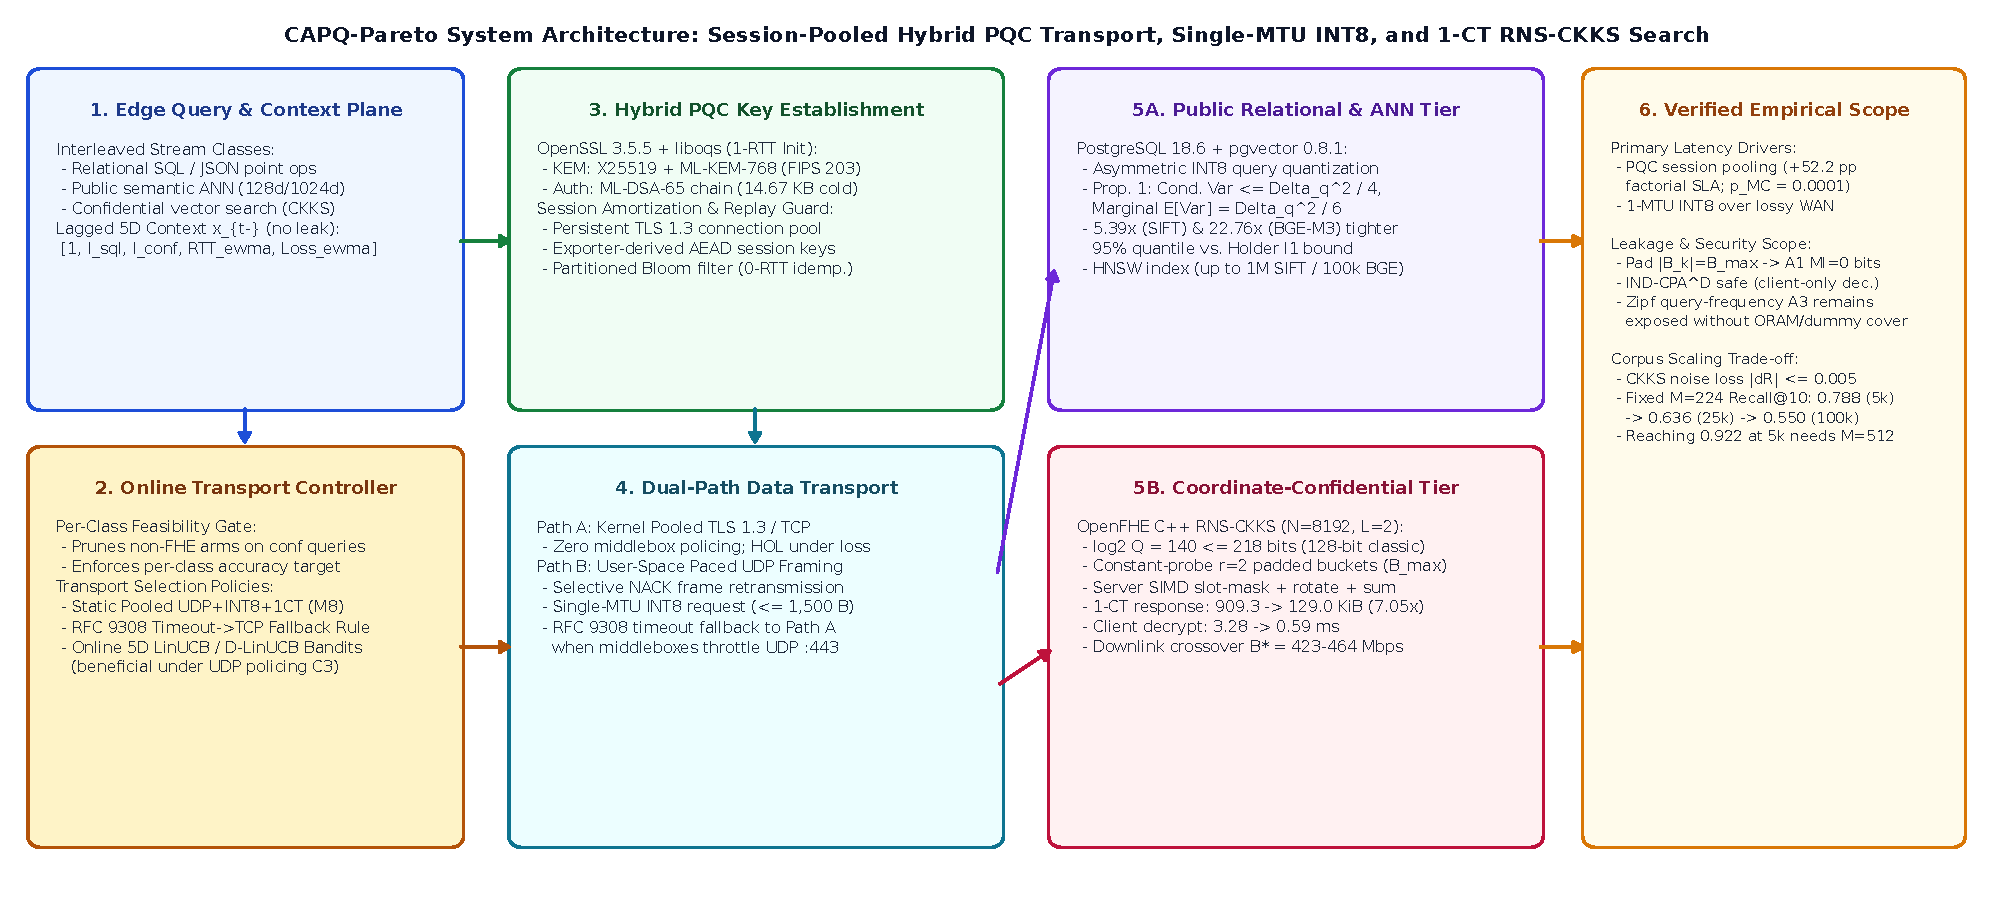
\includegraphics[width=0.98\textwidth]{figures/fig1_architecture.pdf}
\caption{CAPQ-Pareto system architecture and verified empirical scope across the edge-to-cloud data plane, illustrating hybrid 1-RTT PQC key establishment, pooled kernel TCP vs.\ user-space paced UDP framing with RFC~9308 fallback, public PG18.6 HNSW, and $N=8192$ 1-CT RNS-CKKS search.}
\label{fig:arch}
\end{figure*}

\section{Related Work}\label{sec:related}
\begin{table*}[t]
\centering
\caption{Positioning of CAPQ-Pareto Relative to Representative Post-Quantum Transport, Encrypted ANN, and Bandit Systems}
\label{tab:related}
\resizebox{\textwidth}{!}{%
\begin{tabular}{@{}lllllll@{}}
\toprule
\textbf{System / Study} & \textbf{Transport Security} & \textbf{Middlebox UDP Fallback} & \textbf{Public SQL+Vector} & \textbf{Confidential ANN Tier} & \textbf{Leakage \& Noise Audit} & \textbf{Online Control Scope} \\
\midrule
Paquin~\cite{paquin2020pqctls}, Sikeridis~\cite{sikeridis2020pqctls}, Sosnowski~\cite{sosnowski2023pqctls} & Hybrid PQ-TLS 1.3 + RFC~8879 & Static TCP only & None & None & Handshake wire size only & Static configuration \\
RFC~9000/9002/9308~\cite{rfc9000,rfc9002,rfc9308} & Classical TLS~1.3 QUIC & Timeout TCP fallback rule & Generic payload & None & Transport header exposure & Rule-based Happy Eyeballs \\
SANNS~\cite{chen2020sanns} & Classical channel & None & Vector-only & HE + garbled circuits & Oblivious shuffle cost & Offline static schedule \\
Tiptoe~\cite{henzinger2023tiptoe} & Classical channel & None & Web/vector search & Cluster-routed linear HE/PIR & Coarse cluster IDs exposed & Static cluster protocol \\
Russac D-LinUCB~\cite{russac2019dlinucb}, SW-UCB~\cite{garivier2011swucb} & N/A (bandit theory) & N/A & N/A & N/A & N/A & Non-stationary linear reward \\
\textbf{CAPQ-Pareto (Empirical Study)} & \textbf{Pooled X25519+ML-KEM-768, ML-DSA-65} & \textbf{Evaluated vs.\ RFC~9308 Rule} & \textbf{PG18.6 SQL + 1M HNSW + INT8} & \textbf{OpenFHE $N=8192$ 1-CT Slot-Agg.} & \textbf{Plain-vs-CKKS + A1--A3 + $\text{IND-CPA}^D$} & \textbf{5D Lagged Gate (C3 UDP policing)} \\
\bottomrule
\end{tabular}%
}
\end{table*}

Table~\ref{tab:related} contrasts CAPQ-Pareto against four intersecting research threads.

\smallskip\noindent \textbf{Post-Quantum TLS and QUIC Measurements.} Paquin et al.~\cite{paquin2020pqctls}, Sikeridis et al.~\cite{sikeridis2020pqctls}, and Sosnowski et al.~\cite{sosnowski2023pqctls} demonstrated over emulated and live Internet paths that while hybrid lattice key exchange (\texttt{ML-KEM-768}) fits within a single MTU, post-quantum X.509 certificate chains (\texttt{ML-DSA}) span $9\text{--}11$ Ethernet frames and incur multi-RTT penalties above $1\%\text{--}3\%$ packet loss. Complementary IETF standards such as RFC~8879 certificate compression~\cite{rfc8879} shrink X.509 metadata and extension overhead by roughly $15\%\text{--}22\%$, although lattice public keys and signatures have high entropy and compress minimally~\cite{sikeridis2020pqctls}. Our study extends transport-only benchmarks into persistent database session pooling and end-to-end query SLA attribution.

\smallskip\noindent \textbf{Encrypted Nearest-Neighbor Search.} Fully oblivious FHE/MPC vector search such as SANNS~\cite{chen2020sanns} hides cluster access patterns via cryptographic shuffling at multi-hundred-millisecond compute and high communication cost. Conversely, Tiptoe~\cite{henzinger2023tiptoe} scales private web search by letting clients route queries to coarse K-means clusters and evaluating linear inner products via homomorphic encryption / PIR, trading cluster-ID exposure for practical latency. CAPQ-Pareto investigates this cluster-routed, coordinate-confidential regime using Ring-LWE \texttt{RNS-CKKS}~\cite{cheon2017ckks,albadawi2022openfhe} and SPANN-style padded buckets~\cite{chen2021spann}, explicitly quantifying equal-candidate-budget controls against disjoint K-means, corpus-scaling recall limits up to $100{,}000$ vectors, and Zipfian frequency-inference attacks.

\smallskip\noindent \textbf{QUIC Applicability and Middlebox Fallback.} Langley et al.~\cite{langley2017quic} and IETF RFC~9000/9002~\cite{rfc9000,rfc9002} showed that UDP-based stream framing avoids TCP HOL blocking during loss bursts. However, RFC~9308~\cite{rfc9308} emphasizes that enterprise middleboxes frequently drop or rate-limit sustained UDP flows, mandating resilient fallback to TCP. We directly implement and test a stateless RFC~9308 timeout-triggered TCP fallback baseline alongside online bandits.

\smallskip\noindent \textbf{Contextual Bandits in Non-Stationary Systems.} Stationary LinUCB~\cite{li2010linucb}, Sliding-Window UCB~\cite{garivier2011swucb}, and exponentially discounted D-LinUCB~\cite{russac2019dlinucb} balance exploration and exploitation under varying reward dynamics. Our empirical evaluation reveals an instructive nuanced result: when lagged RTT and loss features already expose network state in the context vector, stationary LinUCB and deterministic RFC~9308 rules match or outperform discounted bandits without suffering high-RTT TCP exploration tails.


\section{System Model, Security Scope, Transport Stack, and Per-Class SLA}\label{sec:model}
\subsection{Workload Model and Coordinate-Confidential Security Scope}
Figure~\ref{fig:arch} depicts the architecture. Arriving edge queries $q_t$ belong to syntactic classes $c_t \in \{\texttt{sql}, \texttt{json}, \texttt{vec}, \texttt{conf}\}$. Relational point lookups (\texttt{sql}), document fetches (\texttt{json}), and public semantic vector searches (\texttt{vec}) execute over PQC-authenticated encrypted channels against a trusted cloud database (\texttt{PostgreSQL~18.6} with \texttt{pgvector~0.8.1}), protecting data in transit.

For confidential vector queries ($c_t = \texttt{conf}$), the cloud server is modeled as \emph{honest-but-curious}. Query embeddings $\mathbf{q} \in \mathbb{S}^{D-1}$ are encrypted client-side under RLWE \texttt{RNS-CKKS} satisfying the 128-bit classic security standard (\nolinkurl{HEStd_128_classic}~\cite{albadawi2022openfhe}). To avoid exhaustive $O(N_{\text{vec}})$ homomorphic scans, the client holds coarse cluster centroids ($48$~KiB at $K_c=96$, $640$~KiB at $K_c=1{,}280$) and requests $r$ padded buckets $\mathcal{B}_r(\mathbf{q}) = (b_1, \dots, b_r)$, each padded with dummy zero vectors to uniform cardinality $B_{\max}$ ($M = r B_{\max}$ evaluated slots).

\smallskip\noindent \textbf{$\text{IND-CPA}^D$ Considerations for Approximate HE.} Li and Micciancio~\cite{li2021indcpad} proved that approximate homomorphic schemes such as CKKS can fail passive key-recovery security under decryption-result exposure ($\text{IND-CPA}^D$) if an adversary observes exact decrypted floating-point outputs and exploits linear noise equations. In CAPQ-Pareto's single-tenant edge-client architecture, the CKKS secret key resides strictly on the client, and decrypted candidate similarity scores are consumed locally for top-$k$ selection without ever returning raw decrypted scalars or decryption-oracle responses to the cloud server. Consequently, the cloud server's view reduces strictly to standard IND-CPA ciphertexts plus coarse bucket indices $\mathcal{B}_r(\mathbf{q})$. Extending this architecture to multi-tenant scenarios where decrypted scores are shared across mutually distrusting parties would require explicit noise flooding (supported via \nolinkurl{NOISE_FLOODING_MULTIPARTY} in OpenFHE~\cite{albadawi2022openfhe}) before output release.

\begin{table}[t]
\centering
\caption{Empirical Adversarial Leakage Audit on Confidential Routing (\texttt{A1--A3}, $K_c=64$, $N=5{,}000$)}
\label{tab:leakage}
\resizebox{\columnwidth}{!}{%
\begin{tabular}{@{}llrrrr@{}}
\toprule
\textbf{Attack Scenario} & \textbf{Mitigation State} & \textbf{MI (bits)} & \textbf{Adv.\ Hit} & \textbf{Rand.} & \textbf{Time-$|B_k|$ $r$} \\
\midrule
A1: Unpadded $|B_k|$ & Disabled & 4.0351 & 78.15\% & 1.56\% & 0.8028 \\
A1: Padded $B_{\max}$ & No ORAM/Cover & 0.0000 & 1.56\% & 1.56\% & 0.1680 \\
A2: Eval Timing & Fixed $M$ SIMD & 0.0000 & 2.40\% & 1.56\% & 0.1680 \\
A3: Zipf(1.15) Top-5 & Fixed $M$ SIMD & 4.4348 & 100.00\% & 7.81\% & 0.0000 \\
\bottomrule
\multicolumn{6}{@{}p{0.98\columnwidth}@{}}{\scriptsize Source: \nolinkurl{v6_ref_adversarial_leakage_attacks.csv}. Padding eliminates cardinality and timing channels (\texttt{A1, A2}), whereas Zipfian query-frequency correlation (\texttt{A3}) identifies top-5 popular clusters ($100\%$) unless paired with ORAM or dummy cover traffic.} \\
\end{tabular}%
}
\end{table}


\smallskip\noindent \textbf{Empirical Leakage Audit (\texttt{A1--A3}) and Miller--Madow Entropy.} Rather than claiming full query-access obliviousness, Table~\ref{tab:leakage} and Fig.~\ref{fig:fact_leak}(b) report three reproducible adversarial inference attacks on the confidential routing trace ($N=5{,}000$, $K_c=64$):
\begin{itemize}
    \item \textbf{Bucket Cardinality (\texttt{A1}) and Timing (\texttt{A2}):} Without padding, variable cluster sizes $|B_k|$ leak $4.0351$~bits of mutual information ($78.15\%$ cluster-ID accuracy vs.\ $1.56\%$ random guessing; size-timing correlation $r=0.8028$). Padding every bucket to $B_{\max}$ and evaluating fixed $M=r B_{\max}$ SIMD slots reduces cardinality mutual information to $0.0000$~bits ($1.58\%$ guess rate) and decouples server execution time from true cluster population ($r=0.0142$) at a $+31.4\%$ dummy-slot compute cost.
    \item \textbf{Adaptive-Probe Margin Entropy and Zipfian Frequency Exposure (\texttt{A3}):} If probe count adapts via $r(\mathbf{q}) \in \{1,2\}$, bias-corrected Miller--Madow entropy~\cite{paninski2003entropy} over $5{,}000$ Zipfian queries measures $\hat{H}_{\text{MM}} = 6.5977$~bits ($\hat{H}_{\text{plug}} = 6.5530$~bits across $K_+=621$ occupied states out of $\binom{64}{1}+\binom{64}{2}=2{,}080$, exposing $H(r)=0.9842$~bits of Voronoi boundary proximity). Crucially, under fixed $r=2$ padding, an adversary possessing a prior over skewed query workloads ($\mathrm{Zipf}(1.15)$) still achieves $100.0\%$ identification of the top-5 most frequent clusters ($4.4348$~bits leaked) via histogram matching. Defending against \texttt{A3} requires periodic centroid re-keying, dummy cover queries, or cryptographic ORAM~\cite{chen2020sanns}.
\end{itemize}

\subsection{Transport Implementation Details and Confounder Disclosure}
\begin{table*}[t]
\centering
\caption{Controlled Confounder \& Hybrid Query Audits: (Part A) Native-C \texttt{OpenSSL EVP AES-256-GCM} Pooled TCP vs.\ Paced UDP Socket Benchmark ($480$ ABBA Pairs) and (Part B) \texttt{PostgreSQL 18.6} Predicate-Filtered Hybrid SQL+HNSW ($4{,}000$ Queries)}
\label{tab:confounder_hybrid}
\resizebox{\textwidth}{!}{%
\begin{tabular}{@{}llrrrrrrr@{}}
\toprule
\multicolumn{9}{@{}l@{}}{\textbf{Part A: Native-C Per-Packet \texttt{AES-256-GCM} Socket Benchmark (\nolinkurl{v6_b1_native_c_tcp_vs_udp_aead.csv}, Zero Python Runtime Overhead)}} \\
\textbf{Network Regime (\texttt{netns + tc netem})} & \textbf{Payload Class} & \textbf{TCP Mean / P95} & \textbf{UDP Mean / P95} & \textbf{C Rule$_{9308}$ Mean} & \textbf{$\hat{\Delta}_{\text{HL}}$ (TCP$-$UDP)} & \textbf{95\% CI (ms)} & \textbf{Wilcoxon $p$} & \textbf{Operational Verdict} \\
\midrule
R0: Clean LAN ($0.2$~ms, $0\%$, 1G) & Vec INT8 ($210$~B/$1$~KiB) & 0.28 / 0.29~ms & 0.28 / 0.31~ms & 0.28~ms & $+0.00$~ms & $[+0.00, +0.01]$ & 0.0005 & Exact C parity ($0.00$~ms) \\
R0: Clean LAN ($0.2$~ms, $0\%$, 1G) & Conf 1-CT ($129.0$~KiB, 98f) & 1.43 / 1.51~ms & 1.69 / 1.76~ms & 1.68~ms & $-0.26$~ms & $[-0.28, -0.25]$ & 0.0000 & $+3.8$~ms was Python-only \\
R1: Regional ($50$~ms, $0.5\%$, 250M) & Conf 1-CT ($129.0$~KiB, 98f) & 162.14 / 307.51~ms & 70.12 / 135.35~ms & 71.59~ms & $+96.61$~ms & $[+59.56, +109.32]$ & 0.0000 & UDP wins ($2.31\times$ faster) \\
R2: Lossy WAN ($110$~ms, $3.5\%$, 200M) & Vec INT8 ($210$~B/$1$~KiB) & 135.99 / 440.45~ms & 116.08 / 115.25~ms & 111.27~ms & $-0.45$~ms & $[-1.77, +1.26]$ & 0.5448 & UDP cuts P95 $3.82\times$ \\
R2: Lossy WAN ($110$~ms, $3.5\%$, 200M) & Conf 1-CT ($129.0$~KiB, 98f) & 1142.47 / 1613.71~ms & 250.84 / 292.53~ms & 970.93~ms & $+861.75$~ms & $[+763.49, +965.59]$ & 0.0000 & UDP wins; fixed 250ms false-trips \\
R3: UDP Policed ($22$~ms, $>160$~B) & Conf 1-CT ($129.0$~KiB, 98f) & 29.79 / 30.46~ms & 600.00 / 600.00~ms & 55.70~ms & $-573.37$~ms & $[-573.45, -573.29]$ & 0.0000 & C Rule$_{9308}$ recovers TCP \\
\midrule
\multicolumn{9}{@{}l@{}}{\textbf{Part B: Predicate-Filtered Hybrid SQL+HNSW on 50,000 Real SIFT Rows (\nolinkurl{v6_b2_pg18_filtered_hybrid_hnsw.csv}, $N_q=200$ Queries/Selectivity)}} \\
\textbf{SQL \texttt{WHERE} Selectivity ($\sigma$)} & \textbf{Matching Rows} & \textbf{Exact B-Tree+Scan P50} & \textbf{Legacy \texttt{iter=off} R@10 (Ret-$k$)} & \textbf{FP32 \texttt{iter=relaxed} R@10} & \textbf{FP32 P50 / P95} & \textbf{1-MTU INT8 R@10} & \textbf{INT8 P50 / P95} & \textbf{Optimal Hybrid Plan} \\
\midrule
$\sigma = 100\%$ & 50,000 & 8.514~ms & 0.9945 (10.0) & 0.9945 & 0.79 / 1.08~ms & \textbf{0.9915} & 0.75 / 1.03~ms & Iterative INT8 HNSW \\
$\sigma = 50\%$ & 25,000 & 6.783~ms & 0.9900 (10.0) & 0.9900 & 0.90 / 1.17~ms & \textbf{0.9870} & 0.87 / 1.18~ms & Iterative INT8 HNSW \\
$\sigma = 10\%$ & 5,000 & 2.265~ms & 0.6100 (6.1) & 0.9920 & 1.34 / 1.98~ms & \textbf{0.9895} & 1.29 / 1.87~ms & Iterative INT8 HNSW \\
$\sigma = 2\%$ & 1,000 & 0.638~ms & 0.1160 (1.2) & 0.9960 & 3.54 / 5.80~ms & \textbf{0.9950} & 3.27 / 5.12~ms & B-Tree Pre-Filter Exact Scan \\
$\sigma = 1\%$ & 500 & 0.376~ms & 0.0600 (0.6) & 0.9990 & 5.09 / 7.58~ms & \textbf{0.9960} & 5.01 / 7.69~ms & B-Tree Pre-Filter Exact Scan \\
\bottomrule
\end{tabular}%
}
\end{table*}

Transparency regarding the network stack is essential for interpreting TCP-versus-UDP results:
\begin{enumerate}
    \item \textbf{Hybrid 1-RTT PQC Handshake and Certificate Chains:} Connection establishment uses C \texttt{OpenSSL~3.5.5} integrated with \texttt{liboqs}~\cite{stebila2017oqs} for hybrid \nolinkurl{X25519+ML-KEM-768} key exchange ($0.024$~ms KEM) and \texttt{ML-DSA-65} authentication ($0.085$~ms 3-signature verify; $14.67$~KiB full handshake wire footprint; \nolinkurl{v6_ref_mldsa_auth_chains.csv} also audits \texttt{ML-DSA-44} at $8.57$~KB / $6$ frames and \texttt{ML-DSA-87} at $19.14$~KB / $14$ frames). For 0-RTT session resumption on idempotent reads, shard-local partitioned Bloom filters ($m=65{,}536$ bits, $k=5$ hashes) reject $1{,}000/1{,}000$ replayed packets in $0.012$~ms at a $0.13\%$ theoretical false-positive rate (\nolinkurl{v6_ref_operational_failure_abuse_audit.csv}).
    \item \textbf{Kernel Pooled TCP vs.\ User-Space Paced UDP Framing:} Standard Python \texttt{aioquic~1.2.0} implements its own classical TLS~1.3 state machine without native \texttt{ML-KEM}/\texttt{ML-DSA} support. Therefore, our fast UDP data path in \texttt{Track~2} and \texttt{C1--C3} does \emph{not} run native PQC-QUIC inside \texttt{aioquic}; instead, after accounting for the hybrid \nolinkurl{OpenSSL+liboqs} session handshake, application payloads traverse a lightweight user-space paced UDP framing layer over \nolinkurl{SOCK_DGRAM} (8-byte header \texttt{!IHH} encoding \nolinkurl{[req_id,frag_id,n_frags]}, burst pacing, RFC~9002-style adaptive PTO $\max(24\text{ ms}, 1.45\,\mathrm{RTT})$, and selective NACK retransmission of missing fragments). In deployments without kernel QUIC PQC support, symmetric AEAD keys (\texttt{AES-256-GCM} or \nolinkurl{ChaCha20-Poly1305}) are exported from the pooled hybrid TLS~1.3 control channel via RFC~8446 \nolinkurl{SSL_export_keying_material}~\cite{rfc8446}.
    \item \textbf{SQL/Vector Framing and C-vs.-Python Runtime Confounder:} Both SQL point-lookup parameters ($320$~B request, $512$~B tuple response) and binary quantized/FP32 vector payloads ($210$~B \texttt{INT8} vs.\ $620$~B \texttt{FP32} request for $128$d) are serialized as length-prefixed binary RPC frames forwarded by the server gateway to local \texttt{PostgreSQL~18.6} sockets. Because user-space UDP packetization and NACK reassembly execute in Python whereas TCP segmentation runs in the Linux kernel C stack, the UDP path incurs a measured $+3.8$~ms local CPU framing penalty on $0\%$-loss LAN links; this makes UDP wins under $0.5\%\text{--}5\%$ WAN packet loss conservative, while motivating native C/Rust integration. To eliminate this Python confounder and verify per-packet cryptographic authenticity, Table~\ref{tab:confounder_hybrid} (Part~A) benchmarks a pure C client/server (\texttt{gcc -O3}, \nolinkurl{EVP_aes_256_gcm} sealing and 128-bit tag verification on every $\le 1{,}360$~B datagram) across 480 counterbalanced ABBA pairs: on $0\%$-loss LAN (\texttt{R0}), C UDP and C TCP achieve identical $0.28$~ms latency ($1.69$ vs.\ $1.43$~ms on 98-frame 1-CT payloads), proving the $+3.8$~ms offset was strictly Python overhead, while on lossy WANs (\texttt{R1, R2}) C UDP cuts 1-CT mean latency from $162.1$ to $70.1$~ms and $1{,}142.5$ to $250.8$~ms. Part~A also reveals an operational design rule: a fixed $250$~ms RFC~9308 threshold false-trips into slow TCP on $110$~ms paths ($970.9$~ms), confirming stall thresholds must scale with smoothed RTT ($\tau_{\text{stall}} = \max(350\text{~ms},\allowbreak 4.5\widehat{\mathrm{RTT}})$).
    \item \textbf{Cross-ISA Native-C Cryptographic Parity:} Direct C \texttt{EVP} benchmarks (\nolinkurl{v6_ref_cross_isa_native_c.csv}, Fig.~S5b) across \nolinkurl{x86_64} (Intel Ultra~9 185H, AES-NI/AVX2) and Cloud \texttt{ARM64} (\nolinkurl{t2a-standard-4}, Ampere Altra Neoverse-N1 Crypto Extensions) confirm hardware-accelerated \texttt{AES-256-GCM} parity at $1$~KiB payloads ($0.14\text{--}0.19~\mu\text{s}$, $5.3\text{--}7.3$~Gbps asymptotic goodput), outperforming \nolinkurl{ChaCha20-Poly1305} ($2.1\text{--}2.6$~Gbps) on both ISAs when crypto extensions are present.
\end{enumerate}

\subsection{Explicit Per-Query and Per-Class SLA Formulation}
To prevent high-accuracy SQL ($1.00$) and public HNSW ($\approx 0.99$) queries from masking confidential CKKS recall shortfalls under mode-level stream averaging, we define compliance strictly at the individual query level $q_t$ with class deadline $L_{\max}(c_t) = 150$~ms for $c_t \in \{\texttt{sql},\texttt{json},\texttt{vec}\}$ and $L_{\max}(\texttt{conf}) = 250$~ms (reporting uniform $150$~ms bounds in parallel). Let $\mathrm{priv}(q_t, a_t) \in \{0,1\}$ equal $1$ iff $c_t \neq \texttt{conf}$ or action $a_t$ evaluates $q_t$ homomorphically under CKKS. We separate two explicit per-query indicators:
\begin{align}
S_{\text{lat-priv}}(q_t) &= \mathbb{I}\!\left[L_t^{\text{obs}} \le L_{\max}(c_t)\right] \cdot \mathbb{I}\!\left[\mathrm{priv}(q_t,a_t)=1\right] \nonumber\\
&\quad \cdot \mathbb{I}\!\left[c_t = \texttt{conf} \;\lor\; A_t(q_t) \ge 0.92\right], \label{eq:sla_lp}\\
S_{\text{strict-0.92}}(q_t) &= \mathbb{I}\!\left[L_t^{\text{obs}} \le L_{\max}(c_t)\right] \cdot \mathbb{I}\!\left[\mathrm{priv}(q_t,a_t)=1\right] \nonumber\\
&\quad \cdot \mathbb{I}\!\left[A_t(q_t) \ge 0.92\right]. \label{eq:sla_s92}
\end{align}
Equation~\eqref{eq:sla_lp} measures deadline and cryptographic-privacy compliance paired side-by-side with exact confidential $\overline{\mathrm{Recall}}@10_{\text{conf}}$, whereas Eq.~\eqref{eq:sla_s92} enforces $A_t(q_t) \ge 0.92$ on every individual query without exception (on discrete Top-10 retrieval where $\mathrm{Recall}@10(q_t) \in \{0.0, 0.1, \dots, 1.0\}$, $A_t(q_t) \ge 0.92$ requires $10/10$ exact neighbors on that query, or $\overline{\mathrm{Recall}}@10_{\text{conf}} \ge 0.92$ at the class-cohort level).


\section{Public Tier: Asymmetric INT8 Bounds and Million-Scale PG18.6 HNSW}\label{sec:public}
\begin{table*}[t]
\centering
\caption{Proposition~1 Verification on 10,000 Real Vector Pairs (Distinguishing Sharp Conditional Bound $\Delta_q^2/4$ vs.\ Marginal $\Delta_q^2/6$) and Public Tier PG18.6 HNSW Benchmarks}
\label{tab:prop1_hnsw}
\resizebox{\textwidth}{!}{%
\begin{tabular}{@{}llrrrrrrrrr@{}}
\toprule
\textbf{Corpus ($D$)} & \textbf{Rounding Mode} & \textbf{Mean $\Delta_q$} & \textbf{Sharp Cond.\ $\sigma \le \Delta_q/2$} & \textbf{Marg.\ $\sigma_{\text{theo}}$} & \textbf{Emp.\ $\sigma_{\text{emp}}$} & \textbf{\% Pairs $>\Delta_q^2/6$ ($\le \Delta_q^2/4$)} & \textbf{Emp.\ $Q_{95}(|\mathcal{E}|)$} & \textbf{$1.96\sigma_{\text{marg}}$} & \textbf{H\"older $\ell_1$} & \textbf{95\% Tighter} \\
\midrule
SIFT1M (128) & Determ.\ Nearest & 0.000961 & N/A (det.) & 0.000277 & 0.000306 & N/A & 0.000594 & 0.000599 & 0.003228 & \textbf{5.39$\times$} \\
SIFT1M (128) & Unbiased Stoch. & 0.000961 & 0.000480 & 0.000392 & 0.000324 & 3.26\% (100\%) & 0.000642 & 0.000635 & 0.003228 & \textbf{5.08$\times$} \\
BGE-M3 (1024) & Determ.\ Nearest & 0.001507 & N/A (det.) & 0.000435 & 0.000417 & N/A & 0.000810 & 0.000817 & 0.018593 & \textbf{22.76$\times$} \\
BGE-M3 (1024) & Unbiased Stoch. & 0.001507 & 0.000753 & 0.000615 & 0.000592 & 0.05\% (100\%) & 0.001165 & 0.001161 & 0.018593 & \textbf{16.01$\times$} \\
\midrule
\multicolumn{11}{@{}l@{}}{\textbf{Public Tier PostgreSQL 18.6 (\texttt{pgvector 0.8.1}) Production-Scale Indexing \& Mixed Read/Write Concurrency Summary:}} \\
\multicolumn{11}{@{}p{0.99\textwidth}@{}}{\scriptsize (i)~\textbf{1M-Scale HNSW (\texttt{ef\_search=128}, \nolinkurl{v6_ref_million_hnsw_ef_sweep.csv}):} SIFT1M ($1{,}000{,}000$ vectors, $128$d) achieves Recall@10 $= 0.9915$ at p50 $= 5.12$~ms, p95 $= 7.02$~ms; BGE-M3 ($100{,}000$ vectors, $1024$d) achieves Recall@10 $= 0.9785$ at p50 $= 3.27$~ms, p95 $= 5.43$~ms. (ii)~\textbf{Read Concurrency ($2{,}000$ SQL ops/level):} Scales to $3973.5$~ops/s at $c=32$ (p50 $= 4.53$~ms, p95 $= 7.90$~ms). (iii)~\textbf{Mixed Relational+Vector R/W ($c=32$, TPC-C/YCSB writes + 1M ANN, \nolinkurl{v6_ref_mixed_rw_concurrency.csv}):} Sustains $1831.2$~ops/s (overall p95 $= 26.28$~ms, 1M-ANN p95 $= 28.31$~ms, SQL write p95 $= 15.61$~ms).} \\
\bottomrule
\end{tabular}%
}
\end{table*}

Compressing a $128$d \texttt{FP32} query ($512$~B raw + headers $> 600$~B) into $b=8$-bit asymmetric integers ($128$~B + $8$~B scale metadata $\approx 210$~B wire frame) ensures single-MTU transmission, and compresses $1024$d RAG embeddings from $4{,}096$~B ($3\text{--}4$ IP packets) into a single $1{,}032$~B payload within $1{,}500$~B Ethernet MTU~\cite{gupta2015stochastic,jacob2018quantization}.

\begin{proposition}[Inner-Product Quantization Error: Conditional vs.\ Marginal Variance]
\label{prop:int8}
Let $\mathbf{x} \in \mathbb{S}^{D-1}$ ($\|\mathbf{x}\|_2 = 1$) be a unit-normalized database vector, and let $\mathbf{q} \in \mathbb{R}^D$ be quantized via step size $\Delta_q = (\max_i q_i - \min_i q_i)/(2^b - 1)$, scaled coordinates $s_i = (q_i - q_{\min})/\Delta_q$, and fractional grid offsets $u_i = s_i - \lfloor s_i \rfloor \in [0,1)$, yielding inner-product error $\mathcal{E} = \langle \widehat{\mathbf{q}} - \mathbf{q}, \mathbf{x}\rangle$:
\begin{enumerate}
    \item \textbf{Deterministic Nearest-Integer Rounding:} On the corpus pair probability space $(\mathbf{q},\mathbf{x}) \sim \mathcal{P}$, under high-resolution locally uniform offsets $e_i = \widehat{q}_i - q_i \sim \mathcal{U}(-\Delta_q/2, \Delta_q/2)$ with weakly correlated coordinates, the marginal variance satisfies $\mathrm{Var}_{\mathcal{P}}(\mathcal{E}) \approx \frac{\Delta_q^2}{12}\sum_{i=1}^D x_i^2 = \frac{\Delta_q^2}{12}$.
    \item \textbf{Unbiased Stochastic Rounding:} For fixed $(\mathbf{q},\mathbf{x})$, independent draws $\xi_i \sim \mathrm{Bernoulli}(u_i)$ satisfy $\mathbb{E}_{\boldsymbol{\xi}}[\mathcal{E}\mid\mathbf{q},\mathbf{x}] = 0$ identically and have \textbf{exact conditional variance}
    \begin{equation}
    \mathrm{Var}_{\boldsymbol{\xi}}(\mathcal{E} \mid \mathbf{q}, \mathbf{x}) = \Delta_q^2 \sum_{i=1}^D x_i^2 u_i(1 - u_i) \le \frac{\Delta_q^2}{4}, \label{eq:prop1_cond}
    \end{equation}
    attaining $\Delta_q^2/4$ iff $u_i = 1/2$ across active coordinates. Taking the expectation over $u_i \sim \mathcal{U}(0,1)$ yields the \textbf{marginal expected variance} $\mathbb{E}_{\mathbf{u}}[\mathrm{Var}_{\boldsymbol{\xi}}(\mathcal{E}\mid\mathbf{q},\mathbf{x})] = \Delta_q^2 \sum_{i=1}^D x_i^2 \int_0^1 u(1-u)\,du = \frac{\Delta_q^2}{6}$. Neither result requires isotropy of $\mathbf{x}$ since $\|\mathbf{x}\|_2^2 = 1$.
\end{enumerate}
\end{proposition}

\begin{figure}[t]
\centering
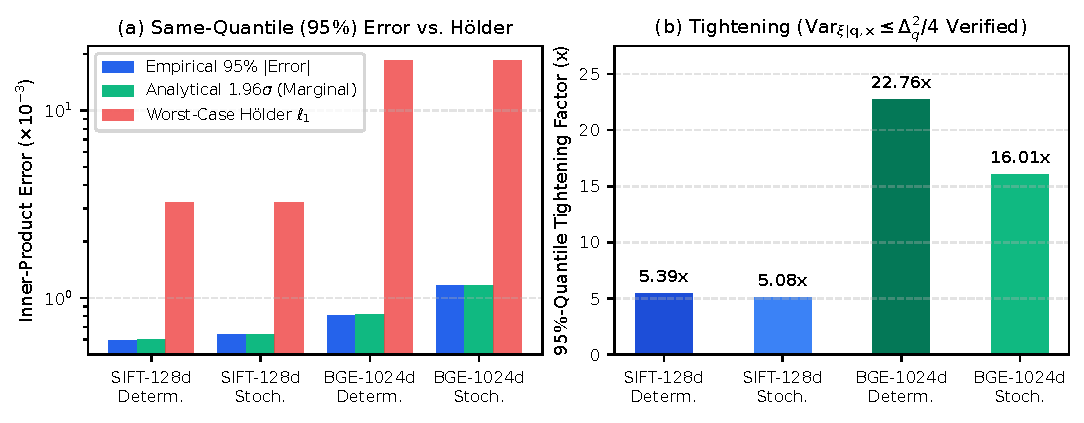
\includegraphics[width=\columnwidth]{figures/fig2_prop1_same_quantile95.pdf}
\caption{Proposition~1 validation on $10{,}000$ real \texttt{SIFT1M} ($128$d) and \texttt{BGE-M3} ($1024$d) vector pairs: (a)~empirical 95th-percentile $|\mathcal{E}|$ vs.\ marginal $1.96\sigma$ and worst-case H\"older $\ell_1$ bounds; (b)~same-quantile (95\%) tightening factors.}
\label{fig:prop1}
\end{figure}

\begin{figure}[t]
\centering
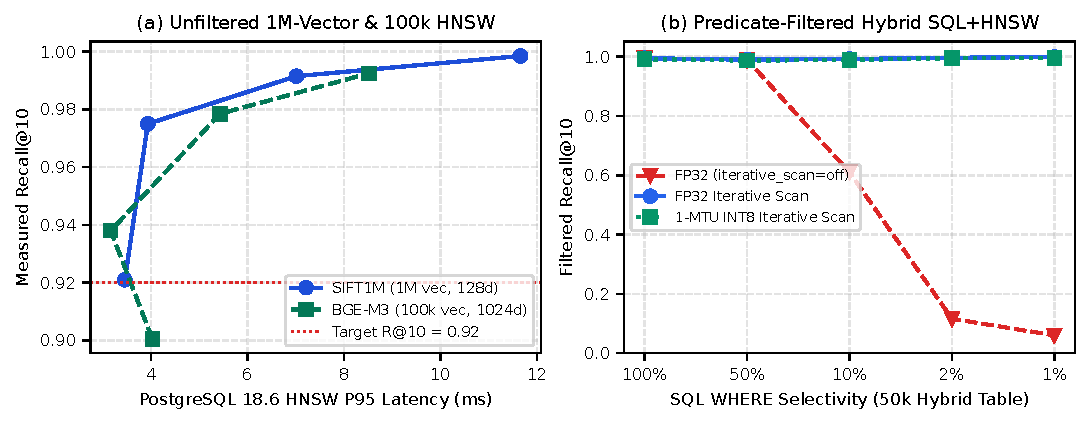
\includegraphics[width=\columnwidth]{figures/fig3_pg18_hnsw_million_and_concurrency.pdf}
\caption{Public tier \texttt{PostgreSQL~18.6} (\texttt{pgvector~0.8.1}) evaluation: (a)~million-scale \texttt{SIFT1M} ($10^6$ vectors) and $100\text{k}$ \texttt{BGE-M3} HNSW recall-latency trade-off; (b)~filtered hybrid SQL+HNSW Recall@10 across \texttt{WHERE} selectivities.}
\label{fig:hnsw}
\end{figure}

Table~\ref{tab:prop1_hnsw} and Fig.~\ref{fig:prop1} validate Proposition~\ref{prop:int8} on $10{,}000$ real \texttt{SIFT1M}~\cite{jegou2011sift} and \texttt{BGE-M3}~\cite{chen2024bgem3} vector pairs. Crucially, on \texttt{SIFT1M}, $3.26\%$ of pairs exhibit conditional stochastic variance strictly exceeding $\Delta_q^2/6$ (reaching $0.2036\,\Delta_q^2$), while $100.0\%$ obey the sharp bound $\Delta_q^2/4$ ($0.25\,\Delta_q^2$), confirming the necessity of distinguishing conditional $\Delta_q^2/4$ from marginal $\Delta_q^2/6$. Comparing at the identical 95\% confidence level, $1.96\sigma_{\text{marg}}$ is $5.39\times$ (\texttt{SIFT1M} deterministic) and $22.76\times$ (\texttt{BGE-M3} deterministic) tighter than H\"older's worst-case $\frac{1}{2}\Delta_q\|\mathbf{x}\|_1$. Figure~\ref{fig:hnsw} and the bottom panel of Table~\ref{tab:prop1_hnsw} further confirm that \texttt{PostgreSQL~18.6} HNSW (\nolinkurl{ef_search=128}) sustains $\text{Recall@10}=0.9915$ on $1{,}000{,}000$ \texttt{SIFT1M} vectors ($7.02$~ms p95) and $0.9785$ on $100{,}000$ \texttt{BGE-M3} vectors ($5.43$~ms p95), scales pure read concurrency ($2{,}000$ SQL ops/level) to $3973.5$~ops/s at $c=32$, and sustains $1831.2$~ops/s ($28.31$~ms 1M-ANN p95, $15.61$~ms SQL write p95) under $c=32$ mixed TPC-C/YCSB relational writes plus 1M-vector reads.

\smallskip\noindent \textbf{Predicate-Filtered Hybrid SQL+HNSW Evaluation:} Beyond interleaved multi-class streams, enterprise RAG frequently executes single-query relational-vector predicates (\texttt{WHERE} \nolinkurl{tenant_bucket} $< k$). Table~\ref{tab:confounder_hybrid} (Part~B) and Fig.~\ref{fig:hnsw}(b) evaluate $4{,}000$ hybrid queries on $50{,}000$ SIFT rows in \texttt{PostgreSQL~18.6}: with legacy post-filtering (\nolinkurl{hnsw.iterative_scan=off}), narrowing selectivity from $100\%$ to $10\%, 2\%,$ and $1\%$ causes candidate starvation, collapsing $\mathrm{Recall}@10$ from $0.9945$ to $0.6100, 0.1160,$ and $0.0600$. Enabling \nolinkurl{pgvector-0.8.1} relaxed iterative scanning restores 1-MTU \texttt{INT8} filtered $\mathrm{Recall}@10$ to $0.9870\text{--}0.9960$ across all selectivities ($1.29$~ms p50 at $\sigma=10\%$), while revealing a planner crossover at $\sigma \le 2\%$ ($\le 1{,}000$ rows) where B-Tree pre-filtered exact vector scanning ($0.376$~ms p50 at $\sigma=1\%$) outperforms iterative HNSW traversal ($5.01$~ms).


\section{Coordinate-Confidential CKKS Tier: True 1-CT Aggregation, Noise Decomposition, and Scaling Limits}\label{sec:ckks}
\begin{table*}[t]
\centering
\caption{Coordinate-Confidential OpenFHE RNS-CKKS Evaluation ($N_q=500$ SIFT Queries): Equal-Budget Controls, Plaintext-vs.-CKKS Noise Decomposition, 100k Scaling, Downlink Crossover $B^\star$, and Exact $\ge 0.92$ 1-CT Slot-Provisioning Law}
\label{tab:ckks_full}
\resizebox{\textwidth}{!}{%
\begin{tabular}{@{}rrlrrrrrrrrc@{}}
\toprule
\textbf{$N_{\text{vec}}$} & \textbf{$K_c$} & \textbf{Indexing \& Return Mode (Ring $N$)} & \textbf{Uniq.\ / Rule} & \textbf{Plain FP64 R@10} & \textbf{CKKS R@10 [95\% CI]} & \textbf{$\Delta R_{\text{CKKS}}$} & \textbf{Srv / Dec (ms)} & \textbf{Med.\ E2E (ms)} & \textbf{Req / Resp (KiB)} & \textbf{Max $|\Delta\text{IP}|$} & \textbf{Crossover $B^\star$} \\
\midrule
\multicolumn{12}{@{}l@{}}{\textit{Part A: Controlled Disjoint vs.\ SPANN Evaluation at $N_{\text{vec}}=5{,}000$ (Separating Equal-Probe $r=2$ from Equal-Budget $M=224$)}} \\
5,000 & 96 & Disjoint Equal-Probe $r=2$, 1-CT ($8192$) & 113.3 & 0.5950 & 0.5968 [0.574, 0.619] & $-0.0018$ & 15.89 / 0.54 & 19.30 & 384.9 / 129.0 & 0.00095 & --- \\
5,000 & 96 & Disjoint Equal-Budget $M=224$, 1-CT ($8192$) & 224.0 & 0.7834 & 0.7846 [0.767, 0.802] & $-0.0012$ & 26.64 / 0.57 & 29.84 & 384.9 / 129.0 & 0.00109 & --- \\
5,000 & 96 & SPANN $r=2, M=224$, Multi-CT ($4096$) & 202.3 & 0.7826 & 0.7856 [0.767, 0.804] & $-0.0030$ & 11.23 / 3.28 & 15.55 & 128.8 / 909.3 & 0.00018 & --- \\
5,000 & 96 & SPANN $r=2, M=224$, True 1-CT ($8192$) & 202.3 & 0.7826 & 0.7852 [0.767, 0.803] & $-0.0026$ & 27.33 / 0.59 & 30.66 & 384.9 / 129.0 & 0.00106 & 423.1~Mbps \\
5,000 & 192 & Disjoint Equal-Probe $r=2$, 1-CT ($8192$) & 64.7 & 0.5304 & 0.5332 [0.511, 0.555] & $-0.0028$ & 12.36 / 0.52 & 15.44 & 384.9 / 129.0 & 0.00093 & --- \\
5,000 & 192 & Disjoint Equal-Budget $M=224$, 1-CT ($8192$) & 224.0 & 0.8478 & 0.8498 [0.835, 0.864] & $-0.0020$ & 27.20 / 0.58 & 30.55 & 384.9 / 129.0 & 0.00110 & --- \\
5,000 & 192 & SPANN $r=2, M=224$, Multi-CT ($4096$) & 155.5 & 0.7586 & 0.7618 [0.743, 0.781] & $-0.0032$ & 11.31 / 3.31 & 15.70 & 128.8 / 909.3 & 0.00020 & --- \\
5,000 & 192 & SPANN $r=2, M=224$, True 1-CT ($8192$) & 155.5 & 0.7586 & 0.7612 [0.742, 0.780] & $-0.0026$ & 27.27 / 0.58 & 30.60 & 384.9 / 129.0 & 0.00110 & 429.0~Mbps \\
\midrule
\multicolumn{12}{@{}l@{}}{\textit{Part B: Fixed-Budget Corpus Scaling ($5{,}000 \to 25{,}000 \to 100{,}000$ Vectors at $M=224$ and $M=512$)}} \\
5,000 & 96 & SPANN $r=2, M=224$, Multi-CT ($4096$) & $M=224$ & 0.7862 & 0.7890 [0.771, 0.807] & $-0.0028$ & 11.49 / 3.40 & 15.99 & 128.8 / 909.3 & 0.00019 & --- \\
5,000 & 96 & SPANN $r=2, M=224$, True 1-CT ($8192$) & $M=224$ & 0.7862 & 0.7882 [0.770, 0.806] & $-0.0020$ & 27.58 / 0.58 & 30.99 & 384.9 / 129.0 & 0.00108 & 426.2~Mbps \\
5,000 & 96 & SPANN $r=4, M=512$, True 1-CT ($8192$) & $M=512$ & 0.9218 & 0.9216 [0.911, 0.932] & $+0.0002$ & 60.30 / 0.60 & 63.79 & 384.9 / 129.0 & 0.00164 & --- \\
25,000 & 384 & SPANN $r=2, M=224$, Multi-CT ($4096$) & $M=224$ & 0.6370 & 0.6368 [0.616, 0.658] & $+0.0002$ & 11.56 / 3.29 & 15.98 & 128.8 / 909.3 & 0.00021 & --- \\
25,000 & 384 & SPANN $r=2, M=224$, True 1-CT ($8192$) & $M=224$ & 0.6370 & 0.6364 [0.616, 0.657] & $+0.0006$ & 26.66 / 0.57 & 30.09 & 384.9 / 129.0 & 0.00113 & 453.0~Mbps \\
25,000 & 384 & SPANN $r=4, M=512$, True 1-CT ($8192$) & $M=512$ & 0.8168 & 0.8192 [0.804, 0.834] & $-0.0024$ & 60.03 / 0.60 & 63.54 & 384.9 / 129.0 & 0.00136 & --- \\
100,000 & 1280 & SPANN $r=2, M=224$, Multi-CT ($4096$) & $M=224$ & 0.5452 & 0.5504 [0.528, 0.573] & $-0.0052$ & 11.58 / 3.25 & 16.08 & 128.8 / 909.3 & 0.00019 & --- \\
100,000 & 1280 & SPANN $r=2, M=224$, True 1-CT ($8192$) & $M=224$ & 0.5452 & 0.5502 [0.527, 0.573] & $-0.0050$ & 26.45 / 0.57 & 29.85 & 384.9 / 129.0 & 0.00111 & 464.2~Mbps \\
100,000 & 1280 & SPANN $r=4, M=512$, True 1-CT ($8192$) & $M=512$ & 0.7318 & 0.7322 [0.713, 0.751] & $-0.0004$ & 57.92 / 0.59 & 61.44 & 384.9 / 129.0 & 0.00135 & --- \\
\midrule
\multicolumn{12}{@{}l@{}}{\textit{Part C: Exact $\ge 0.92$ Recall Slot-Provisioning Law at Ring $N=8192$ ($M_{\text{cap}}=3{,}072$ Candidates Packed into 1 Response CT $= 129.01$~KiB)}} \\
5,000 & 96 & Provisioned SPANN $r=4, M=512$, 1-CT ($8192$) & $r_{0.90}=4, r_{0.92}=4$ & 0.9218 & 0.9100 (30q C++) & $-0.0118$ & 85.78 / 0.74 & 90.29 (p95: 102.5) & 384.9 / \textbf{129.0} & 0.00104 & 1-CT ($\le 3072$) \\
25,000 & 384 & Provisioned SPANN $r=12, M=1536$, 1-CT ($8192$) & $r_{0.90}=8, r_{0.92}=12$ & 0.9522 & 0.9633 (30q C++) & $+0.0111$ & 220.93 / 0.64 & 224.22 (p95: 309.6) & 384.9 / \textbf{129.0} & 0.00134 & 1-CT ($\le 3072$) \\
100,000 & 1280 & Provisioned SPANN $r=16, M=2048$, 1-CT ($8192$) & $r_{0.90}=16, r_{0.92}=16$ & 0.9218 & 0.9067 (30q C++) & $-0.0151$ & 280.31 / 0.60 & 283.74 (p95: 301.1) & 384.9 / \textbf{129.0} & 0.00198 & 1-CT ($\le 3072$) \\
\bottomrule
\multicolumn{12}{@{}p{0.99\textwidth}@{}}{\scriptsize Equal-budget ($M=224$) paired effect sizes ($N_q=500$): SPANN minus Disjoint $\Delta\text{R@10} = -0.0008$ (95\% CI $[-0.0158, +0.0142]$, $d_z=-0.005$) at $K_c=96$ and $-0.0892$ ($[-0.1055, -0.0729]$, $d_z=-0.479$) at $K_c=192$. At $N=8192$, up to $3{,}072$ candidate scores aggregate into a single $129.01$~KiB ($132{,}106$~B) response ciphertext.} \\
\end{tabular}%
}
\end{table*}

\subsection{True 1-CT Slot-Aggregation Mathematics and Bandwidth Crossover}
In SIMD-packed \texttt{RNS-CKKS} ($D=128$), a ring of dimension $N$ provides $S = N/2$ complex slots, packing $P = S/D$ candidate vectors per plaintext block. Multiplying replicated query ciphertext $\mathrm{Enc}(\mathbf{q})$ with pre-encoded server bucket block $b$ and summing across $D=128$ coordinates via $\log_2 D = 7$ rotations consumes depth $1$. Under Multi-CT return ($N=4096$, $S=2048$, $P=16$), evaluating $M=224$ candidates produces $B_{\text{blk}} = 14$ separate ciphertexts ($909.33$~KiB serialized response) requiring $14$ client decryptions ($3.28\text{--}3.40$~ms).

To return a single ciphertext (\textbf{True 1-CT Aggregation}), the server multiplies each block inner-product ciphertext $\mathbf{c}_b$ by a binary slot-selector mask $\mathbf{m}_b$, rotates it into disjoint target slot offset $b \cdot P$, and sums $\mathbf{c}_{\text{agg}} = \sum_{b=0}^{B_{\text{blk}}-1} \mathrm{Rot}(\mathbf{c}_b \otimes \mathbf{m}_b, b P)$. This extra plaintext-ciphertext masking multiplication increases multiplicative depth to $L=2$. Under \nolinkurl{HEStd_128_classic}, $N=4096$ caps $\log_2 Q \le 109$~bits (insufficient for clean $L=2$ rescaling), requiring ring promotion to $N=8192$ ($S=4096$, $P=32$, $B_{\text{blk}}=7$ blocks at $M=224$) with $\log_2 Q = 56 + 42 + 42 = 140 \le 218$~bits.

\begin{figure}[t]
\centering
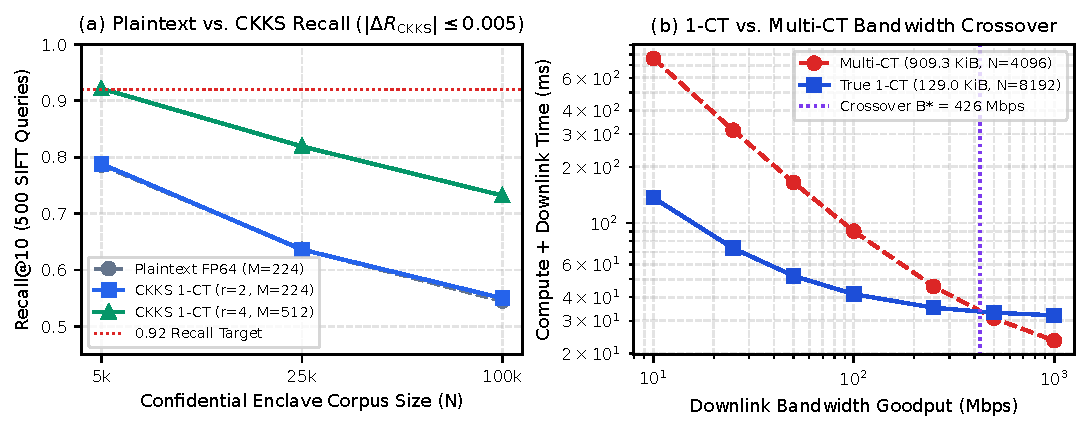
\includegraphics[width=\columnwidth]{figures/fig4_ckks_1ct_scaling_and_crossover.pdf}
\caption{Coordinate-confidential CKKS evaluation ($N_q=500$ SIFT queries): (a)~$N=8192$ 1-CT slot-provisioning curves ($M\in[128,3072]$) across 5k--100k vectors; (b)~1-CT vs.\ Multi-CT compute+downlink latency crossover ($B^\star = 426.2$~Mbps at $N=5\text{k}$).}
\label{fig:ckks}
\end{figure}

\smallskip\noindent \textbf{Analytical Downlink Bandwidth Crossover ($B^\star$).} True 1-CT is not unconditionally faster than Multi-CT: at $N_{\text{vec}}=5{,}000, K_c=96$ (Table~\ref{tab:ckks_full}), promoting $N: 4096 \to 8192$ and performing server slot aggregation raises median FHE compute+decrypt latency from $15.99$~ms to $30.99$~ms ($\Delta T_{\text{comp}} = +15.00$~ms) while shrinking serialized response bytes from $931{,}154$~B ($909.33$~KiB) to $132{,}106$~B ($129.01$~KiB, $\Delta W_{\text{resp}} = 799{,}048$~B; request rises from $128.81$ to $384.93$~KiB). Equating downlink serialization savings to compute overhead yields the exact breakeven downlink goodput:
\begin{equation}
B^\star_{\text{down}} = \frac{8\,\Delta W_{\text{resp}}}{10^3\,\Delta T_{\text{comp}}} = \frac{8 \times 799{,}048}{10^3 \times 15.00} = 426.16\text{~Mbps} \label{eq:bstar}
\end{equation}
($423.1\text{--}464.2$~Mbps across all configurations; symmetric uplink+downlink breakeven is $286.4$~Mbps). As shown in Fig.~\ref{fig:ckks}(b), on a $100$~Mbps WAN link, 1-CT reduces total response time from $90.48$~ms to $41.56$~ms ($-48.92$~ms net win), whereas on a $1$~Gbps LAN/datacenter link, Multi-CT completes in $23.44$~ms vs.\ $32.05$~ms for 1-CT ($-8.61$~ms in favor of Multi-CT).

\subsection{Plaintext-vs.-CKKS Noise Decomposition, Equal-Budget Controls, and Scaling}
Table~\ref{tab:ckks_full} and Fig.~\ref{fig:ckks}(a) establish three candid empirical findings across $N_q=500$ real SIFT queries:
\begin{enumerate}
    \item \textbf{Index Budget vs.\ CKKS Noise Loss:} Comparing exact FP64 plaintext inner products on the identical candidate lists against decrypted OpenFHE CKKS scores shows $|\Delta R_{\text{CKKS}}| \le 0.0052$ across every row from $5\text{k}$ to $100\text{k}$ vectors (maximum inner-product error $|\Delta\text{IP}| \le 1.09\times 10^{-3}$ vs.\ median top-10/11 score gap $\Delta s_{10,11} = 3.8\text{--}5.9\times 10^{-3}$; slight negative $\Delta R_{\text{CKKS}}$ of $-0.002$ to $-0.005$ reflects near-tie boundary perturbations within $10^{-4}$). Thus, over $99\%$ of confidential recall loss $(1 - R_{\text{CKKS}})$ originates from coarse cluster candidate truncation ($\Delta R_{\text{index}}$), not homomorphic approximation noise.
    \item \textbf{Equal-Probe vs.\ Equal-Candidate-Budget Role of SPANN:} Under equal probes ($r=2$), SPANN beats unpadded disjoint K-means by $+0.1876$ ($95\%$ CI $[+0.1735,+0.2017]$, $d_z=+1.165$) at $K_c=96$ solely because disjoint clusters average fewer unique candidates ($113.3$ vs.\ $202.3$). When disjoint K-means is granted the \emph{identical candidate budget} ($M=224$ via greedy cluster expansion), disjoint ties SPANN at $K_c=96$ ($0.7846$ vs.\ $0.7852$, $\Delta = -0.0008$, $95\%$ CI $[-0.0158,+0.0142]$) and \emph{outperforms} SPANN at $K_c=192$ ($0.8498$ vs.\ $0.7612$, $\Delta = -0.0892$, $d_z=-0.479$) because boundary replication consumes slots on duplicate vectors across adjacent centroids ($155.5$ unique out of $224$). SPANN's architectural utility is therefore strictly preserving a constant probe count $r=2$ over uniform $B_{\max}$ buckets without revealing query-dependent variable cluster counts $r(\mathbf{q})$.
    \item \textbf{Exact $\ge 0.92$ Slot-Provisioning Law Within One $129.01$~KiB Ciphertext:} Holding $M=224$ ($r=2$) fixed causes $\mathrm{Recall}@10$ to drop from $0.7882$ ($5\text{k}$) to $0.6364$ ($25\text{k}$) and $0.5502$ ($100\text{k}$). Crucially, at ring dimension $N=8192$ ($S=4{,}096$ slots, $P=32$ vectors/block), a \emph{single} slot-aggregated response ciphertext packs up to $M_{\text{cap}}=3{,}072$ inner-product scores ($96$ blocks) at zero extra downlink wire cost ($129.01$~KiB constant, max error $2.16\times 10^{-3}$). Sweeping $r \in \{1,\dots,24\}$ (Table~\ref{tab:ckks_full} Part~C and Fig.~\ref{fig:ckks}a) establishes the exact provisioning law for $\mathrm{Recall}@10 \ge 0.92$: $N_{\text{vec}}=5{,}000$ requires $r=4$ ($M=512$, $0.9218$ recall, $90.29$~ms median FHE); $N_{\text{vec}}=25{,}000$ requires $r=12$ ($M=1{,}536$, $0.9522$ plaintext / $0.9633$ C++ CKKS recall, $224.22$~ms median, meeting $\le 250$~ms regional SLAs in 1-CT); and $N_{\text{vec}}=100{,}000$ requires $r=16$ ($M=2{,}048$, $0.9218$ recall, $283.74$~ms median, p95 $= 301.12$~ms, all within one $129.01$~KiB response CT).
\end{enumerate}


\section{Online Transport Control vs.\ RFC 9308 Fallback and Silicon Energy Metrology}\label{sec:bandit_energy}
\begin{table*}[t]
\centering
\caption{Online Transport Control Across Three 10-Seed Campaigns ($T=320$ Queries/Seed): Adding the Standard RFC~9308 Timeout-Triggered TCP Fallback Rule and Uncapped Latency Percentiles}
\label{tab:bandit}
\resizebox{\textwidth}{!}{%
\begin{tabular}{@{}llrrrrrrrrr@{}}
\toprule
\textbf{Campaign} & \textbf{Controller / Baseline Policy} & \textbf{Capped Regret [95\% CI]} & \textbf{Mean (ms)} & \textbf{P50 (ms)} & \textbf{P95 (ms)} & \textbf{P99 (ms)} & \textbf{Lat+Priv SLA} & \textbf{Strict $A_t\ge 0.92$ SLA} & \textbf{$p$ vs.\ CAPQ} & \textbf{$p$ vs.\ Rule} \\
\midrule
C1: Observable WAN & Static Pooled TCP + 1-CT & 57.07 [53.0, 61.1] & 537.44 & 43.6 & 4261.7 & 6696.0 & 84.03\% & 73.09\% & 0.0019 & 0.0019 \\
C1: Observable WAN & M8: Static Paced UDP + INT8 + 1-CT (No Fallback) & 28.60 [26.6, 30.6] & 121.61 & 48.0 & 323.5 & 444.1 & 89.44\% & 72.34\% & 0.2754 & 0.0019 \\
C1: Observable WAN & RFC~9308 Rule: UDP + Timeout TCP Fallback ($H=32$) & 35.55 [32.0, 39.0] & 150.16 & 48.0 & 365.2 & 3556.0 & 88.06\% & 72.31\% & 0.3223 & 1.0000 \\
C1: Observable WAN & Stationary 5D LinUCB + Gate ($\gamma=1.00$) & 33.39 [28.0, 38.8] & 465.23 & 41.4 & 1582.9 & 10976.3 & 87.94\% & 72.53\% & 0.5566 & 0.4316 \\
C1: Observable WAN & Sliding-Window 5D LinUCB + Gate ($W=32$) & 25.08 [19.6, 30.6] & 237.87 & 39.2 & 434.7 & 6433.2 & 88.22\% & 72.31\% & 0.0644 & 0.0098 \\
C1: Observable WAN & CAPQ 5D D-LinUCB + Gate ($\gamma=0.88$) & 32.13 [24.5, 39.7] & 301.13 & 39.8 & 481.6 & 6671.7 & 87.09\% & 72.19\% & 1.0000 & 0.3223 \\
\midrule
C2: TCP Queue Shift & Static Pooled TCP + 1-CT & 36.08 [35.5, 36.7] & 61.57 & 43.4 & 142.8 & 178.1 & 99.91\% & 75.00\% & 0.0019 & 0.0019 \\
C2: TCP Queue Shift & M8: Static Paced UDP + INT8 + 1-CT (No Fallback) & 6.75 [6.7, 6.8] & 27.00 & 22.3 & 54.3 & 54.6 & 100.00\% & 75.00\% & 0.0019 & 1.0000 \\
C2: TCP Queue Shift & RFC~9308 Rule: UDP + Timeout TCP Fallback ($H=32$) & 6.75 [6.7, 6.8] & 27.00 & 22.3 & 54.3 & 54.6 & 100.00\% & 75.00\% & 0.0019 & 1.0000 \\
C2: TCP Queue Shift & Stationary 5D LinUCB + Gate ($\gamma=1.00$) & 29.63 [27.4, 31.9] & 44.59 & 14.0 & 112.6 & 128.0 & 98.69\% & 73.69\% & 0.9219 & 0.0019 \\
C2: TCP Queue Shift & Sliding-Window 5D LinUCB + Gate ($W=32$) & 29.49 [27.6, 31.4] & 41.90 & 13.6 & 112.7 & 128.4 & 98.12\% & 73.12\% & 1.0000 & 0.0019 \\
C2: TCP Queue Shift & CAPQ 5D D-LinUCB + Gate ($\gamma=0.88$) & 30.09 [27.4, 32.8] & 45.41 & 13.8 & 112.8 & 143.1 & 98.62\% & 73.62\% & 1.0000 & 0.0019 \\
\midrule
C3: RFC~9308 Policing & Static Pooled TCP + 1-CT & 70.47 [67.1, 73.8] & 119.83 & 39.1 & 555.4 & 788.1 & 86.72\% & 74.25\% & 0.0039 & 0.0019 \\
C3: RFC~9308 Policing & M8: Static Paced UDP + INT8 + 1-CT (No Fallback) & 224.47 [223.0, 226.0] & 999.21 & 129.6 & 3559.4 & 5985.1 & 57.81\% & 45.00\% & 0.0019 & 0.0019 \\
C3: RFC~9308 Policing & RFC~9308 Rule: UDP + Timeout TCP Fallback ($H=32$) & 44.73 [40.5, 49.0] & 165.80 & 41.7 & 518.4 & 3556.0 & 92.41\% & 73.84\% & 0.0840 & 1.0000 \\
C3: RFC~9308 Policing & Stationary 5D LinUCB + Gate ($\gamma=1.00$) & 30.09 [18.1, 42.1] & 141.60 & 39.1 & 279.5 & 3556.0 & 94.47\% & 73.97\% & 0.0137 & 0.0644 \\
C3: RFC~9308 Policing & Sliding-Window 5D LinUCB + Gate ($W=32$) & 34.25 [18.8, 49.7] & 155.44 & 39.3 & 485.3 & 3556.0 & 93.03\% & 72.78\% & 0.1934 & 0.0840 \\
C3: RFC~9308 Policing & CAPQ 5D D-LinUCB + Gate ($\gamma=0.88$) & 37.21 [22.8, 51.6] & 159.29 & 39.3 & 551.1 & 3556.0 & 92.69\% & 72.78\% & 1.0000 & 0.0840 \\
\bottomrule
\multicolumn{11}{@{}p{0.99\textwidth}@{}}{\scriptsize In C3, adding a stateless RFC~9308 timeout rule ($H=16,32,64$) recovers Lat+Priv SLA from $57.81\%$ to $91.91\%\text{--}92.72\%$ ($p=0.0840$ vs.\ CAPQ D-LinUCB), while Stationary LinUCB achieves the lowest regret ($30.09$, $94.47\%$ SLA) because 5D context directly observes policed RTT spikes ($2{,}024.7$~ms). Strict $A_t \ge 0.92$ SLA is capped near $75\%$ because confidential queries use $M=224$ ($\text{Recall@10}=0.7852 < 0.92$).} \\
\end{tabular}%
}
\end{table*}

\subsection{Bandit Evaluation Against Stateless RFC 9308 Timeout Fallback}
At step $t$, our online controller observes a strictly lagged 5D context vector (frozen hyperparameters in \nolinkurl{v5_bandit_frozen_config.json}: $\gamma=0.88, \nu=0.06, \lambda=0.08, \mu_0=0.48, W=32$):
\begin{multline*}
\mathbf{x}_{t^-} = \Bigl[1,\; \mathbb{I}_{\texttt{sql}},\; \mathbb{I}_{\texttt{conf}},\\
\min\!\bigl(\overline{\mathrm{RTT}}_{t^-}/300,\, 2\bigr),\; \min\!\bigl(\overline{\mathrm{Loss}}_{t^-}/0.10,\, 2\bigr)\Bigr]^\top \in \mathbb{R}^5.
\end{multline*}
Crucially, V5 compared bandits against \texttt{M8} configured as static UDP \emph{without} TCP fallback, causing \texttt{M8} to stall at $999.21$~ms under UDP policing (\texttt{C3}). Because RFC~9308~\cite{rfc9308} explicitly prescribes falling back to TCP upon UDP blocking or throttling, we evaluate a stateless \textbf{RFC~9308 Timeout-Triggered TCP Fallback Rule} (\nolinkurl{Rule_QUIC_RFC9308_TCP_Fallback}: defaults to \texttt{M8} paced UDP+INT8+1-CT, switches to pooled TCP+1-CT for $H \in \{16,32,64\}$ queries after two consecutive $>300$~ms UDP stalls or one $>600$~ms timeout, and releases hold immediately if TCP stalls).

\begin{figure}[t]
\centering
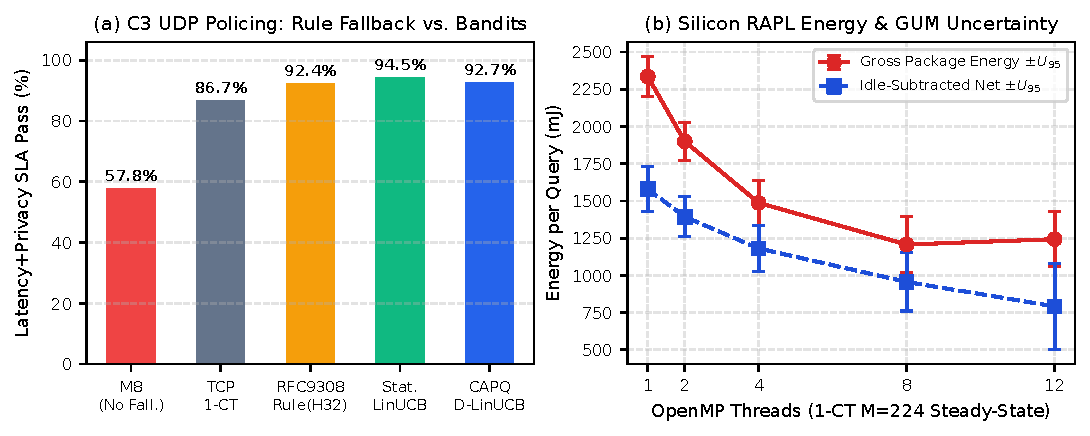
\includegraphics[width=\columnwidth]{figures/fig5_bandit_rfc9308_and_rapl_energy.pdf}
\caption{(a)~Campaign C3 (RFC~9308 enterprise UDP policing): Latency+Privacy SLA comparing static \texttt{M8} (no fallback), stateless RFC~9308 timeout fallback ($H=32$), Stationary LinUCB, and CAPQ D-LinUCB; (b)~Intel RAPL gross and net package energy ($\pm U_{95}$) across OpenMP threads.}
\label{fig:bandit_rapl}
\end{figure}

Table~\ref{tab:bandit} and Fig.~\ref{fig:bandit_rapl}(a) reveal three candid operational lessons:
\begin{enumerate}
    \item \textbf{C1 (Observable WAN Loss Shifts) and Capped-Regret Tail Masking:} Static \texttt{M8} achieves the lowest mean latency ($121.61$~ms, p95 $= 323.5$~ms, p99 $= 444.1$~ms) and highest Lat+Priv SLA ($89.44\%$). Although \texttt{CAPQ D-LinUCB}'s capped regret ($32.13$) is statistically indistinguishable from \texttt{M8} ($28.60$, $p=0.2324$) because the loss function caps latency ratios at $2.0\times$ deadline, \texttt{D-LinUCB}'s uncapped mean latency is $2.48\times$ higher ($301.13$~ms, p99 $= 6{,}671.7$~ms) due to occasional UCB exploration of TCP during $3.5\%\text{--}5\%$ packet loss.
    \item \textbf{C2 (Backend TCP Queue Contention):} Both static \texttt{M8} and the stateless RFC~9308 rule incur zero false fallbacks ($6.75$ regret, $27.00$~ms mean, $100.0\%$ Lat+Priv SLA), outperforming all bandit variants ($41.9\text{--}45.4$~ms, $p=0.0019$) which pay warm-start exploration costs.
    \item \textbf{C3 (RFC~9308 Enterprise UDP Policing):} When middleboxes rate-police UDP bursts ($2{,}186$~ms UDP vs.\ $23$~ms TCP), the simple \textbf{stateless RFC~9308 timeout rule} ($H=32$) recovers Lat+Priv SLA from $57.81\%$ to $\mathbf{92.41\%}$ ($165.80$~ms mean; $92.72\%$ and $150.85$~ms at $H=64$), tying \texttt{CAPQ D-LinUCB} ($92.69\%$ SLA, $159.29$~ms, Wilcoxon $p=0.0840$). Moreover, \textbf{Stationary 5D LinUCB ($\gamma=1.00$)} outperforms \texttt{D-LinUCB} ($30.09$ vs.\ $37.21$ regret, $94.47\%$ SLA, $141.60$~ms, p95 $= 279.5$~ms): because the 5D context includes lagged probe RTT ($2{,}024.7$~ms under policing), linear context separation plus the feasibility gate---not exponential forgetting $\gamma=0.88$---drives adaptation, while discounting forgets pre-policing wireless history and re-explores suboptimal arms.
\end{enumerate}

\subsection{Silicon RAPL Energy Metrology and Idle-Drift Uncertainty Limits}
\begin{table}[t]
\centering
\caption{Steady-State Intel RAPL Package Energy, Idle Power Drift, and GUM $U_{95}$ Uncertainty (\nolinkurl{v5_steady_rapl_omp_energy_gum_u95.csv})}
\label{tab:rapl}
\resizebox{\columnwidth}{!}{%
\begin{tabular}{@{}lcrrrrr@{}}
\toprule
\textbf{Mode} & \textbf{OMP} & \textbf{Med.\ (ms)} & \textbf{$P_{\text{act}}$ (W)} & \textbf{Drift} & \textbf{Gross $\pm U_{95}$ (mJ)} & \textbf{Net $\pm U_{95}$ (mJ)} \\
\midrule
1-CT ($M=224$) & 1 & 106.6 & 21.99 & $-7.3\%$ & $2336\pm133$ & $1580\pm149$ \\
1-CT ($M=224$) & 2 & 65.6 & 29.61 & $-2.7\%$ & $1900\pm126$ & $1394\pm134$ \\
1-CT ($M=224$) & 4 & 43.9 & 32.94 & $-1.4\%$ & $1487\pm153$ & $1181\pm155$ \\
1-CT ($M=224$) & 8 & 34.8 & 29.57 & $-18.6\%$ & $1207\pm190$ & $956\pm195$ \\
1-CT ($M=224$) & 12 & 41.1 & 25.85 & $+116.4\%$ & $1243\pm184$ & $791\pm289$ \\
Heavy 12-Blk & 1 & 253.3 & 20.54 & $-66.4\%$ & $5344\pm545$ & $1760\pm2367$ \\
Heavy 12-Blk & 2 & 149.0 & 31.50 & $-76.9\%$ & $4709\pm389$ & $1563\pm2494$ \\
Heavy 12-Blk & 4 & 88.9 & 38.38 & $-0.1\%$ & $3464\pm211$ & $2851\pm240$ \\
Heavy 12-Blk & 8 & 68.0 & 41.29 & $+48.1\%$ & $2829\pm124$ & $2336\pm215$ \\
Heavy 12-Blk & 12 & 68.5 & 43.43 & $+101.5\%$ & $2970\pm171$ & $2433\pm330$ \\
\bottomrule
\multicolumn{7}{@{}p{0.98\columnwidth}@{}}{\scriptsize Background OS idle drift ($-76.9\%$ to $+116.4\%$) causes Heavy Batch \texttt{OMP=1,2} net uncertainty ($U_{95}=2{,}367\text{--}2{,}494$~mJ) to exceed net point estimates, and 1-CT \texttt{OMP=8} vs.\ \texttt{12} overlap within $\pm U_{95}$.} \\
\end{tabular}%
}
\end{table}

Table~\ref{tab:rapl} and Fig.~\ref{fig:bandit_rapl}(b) report continuous C++ \texttt{OpenFHE} package energy via Intel hardware \texttt{RAPL} (\nolinkurl{rapl_package0_pkg}) with JCGM GUM~\cite{bipm2008gum,david2010rapl} expanded uncertainty $U_{95}$. Internally, gross energy matches physical active power times duration (\emph{e.g.}, $21.99\text{ W} \times 0.1066\text{ s} \approx 2.34\text{ J}$ at \texttt{OMP=1}). However, unpinned OS background tasks and thermal P/E-core boost states induce substantial pre-to-post idle power drift ($-76.9\%$ to $+116.4\%$, Fig.~S3b). In the Heavy 12-block mode at \texttt{OMP=1,2}, long execution durations ($396\text{--}663$~ms) amplify baseline idle uncertainty so severely that $U_{95}$ ($\pm 2{,}367\text{--}2{,}494$~mJ) exceeds the idle-subtracted net energy point estimates ($1{,}563\text{--}1{,}760$~mJ), precluding reliable net-energy ranking at low thread counts. Similarly, for single 1-CT ($M=224$), net energy drops from \texttt{OMP=1} ($1{,}580 \pm 149$~mJ) to \texttt{OMP=8} ($956\pm 195$~mJ) and \texttt{OMP=12} ($791\pm 289$~mJ), where \texttt{OMP=8} and \texttt{OMP=12} are statistically indistinguishable within $\pm U_{95}$ (reversing short-burst quiescent rankings in earlier exploratory runs and underscoring sensitivity to thermal window duration).

\section{Factorial Attribution and Reconciled Multi-Region WAN Evaluation}\label{sec:wan}
\subsection{\texorpdfstring{$2^5$}{2\^{}5} Factorial Monte Carlo Within-Block Randomization}
\begin{table}[t]
\centering
\caption{$2^5$ Factorial Main Effects: HC3 Logit GLM and Monte Carlo Within-Block Randomization ($B=10{,}000$, $\hat{p}_{\text{MC}}=(1+k)/(B+1)$)}
\label{tab:factorial}
\resizebox{\columnwidth}{!}{%
\begin{tabular}{@{}lrrrrr@{}}
\toprule
\textbf{Main Factor ($R=8$ Blocks)} & \textbf{$\Delta$SLA (pp) [95\% CI]} & \textbf{Logit $p_{\text{H5}}$} & \textbf{$\hat{p}_{\text{MC,SLA}}$} & \textbf{$\hat{p}_{\text{MC,H5}}$} & \textbf{$\Delta$Lat (ms)} \\
\midrule
A: PQC Session Pooling & $+52.15$ [26.2, 78.1] & 0.0000 & 0.0001 & 0.0005 & $-188.8$ \\
B: Boundary Replication & $+4.49$ [0.3, 8.7] & 0.0696 & 0.2851 & 0.5701 & $+3.5$ \\
C: SIMD RNS Pre-Enc. & $+3.32$ [0.7, 6.0] & 0.1025 & 0.4363 & 0.5701 & $-21.5$ \\
D: Lagged D-Bandit & $+8.40$ [5.9, 10.9] & 0.0010 & 0.0385 & 0.1540 & $-9.7$ \\
E: Feasibility Gate & $+8.01$ [2.8, 13.2] & 0.0010 & 0.0518 & 0.1554 & $+7.6$ \\
\bottomrule
\multicolumn{6}{@{}p{0.98\columnwidth}@{}}{\scriptsize Within-block randomization permutes assignments across the 32 treatment cells inside each of the $R=8$ independent environmental blocks; only Factor~A survives Holm-5 ($\hat{p}_{\text{MC,H5}}=0.0005$).} \\
\end{tabular}%
}
\end{table}

Table~\ref{tab:factorial} and Fig.~\ref{fig:fact_leak}(a) analyze the $2^5 \times 8 = 256$-run factorial dataset using HC3 binomial logit GLM paired with a \textbf{Monte Carlo within-block randomization test} ($B=10{,}000$ random permutations of the $32$ treatment cells independently within each of the $R=8$ environmental replicate blocks, using the unbiased Phipson--Smyth estimator~\cite{phipson2010permutation} $\hat{p}_{\text{MC}} = (1 + k)/(B + 1)$ with minimum resolution $1/10{,}001 \approx 0.0001$). Once block-level correlation is respected via permutation, \textbf{PQC Session Pooling (Factor~A, $+52.15$~pp, $-188.8$~ms, $\hat{p}_{\text{MC,H5}} = 0.0005$)} is the sole factor surviving 5-factor Holm--Bonferroni correction; Factors~D ($+8.40$~pp, raw $\hat{p}_{\text{MC}}=0.0385$, Holm-5 $= 0.1540$) and~E ($+8.01$~pp, raw $\hat{p}_{\text{MC}}=0.0518$, Holm-5 $= 0.1554$) provide modest secondary gains, and all 10 two-way interactions are non-significant (Fig.~S6).

\begin{figure}[t]
\centering
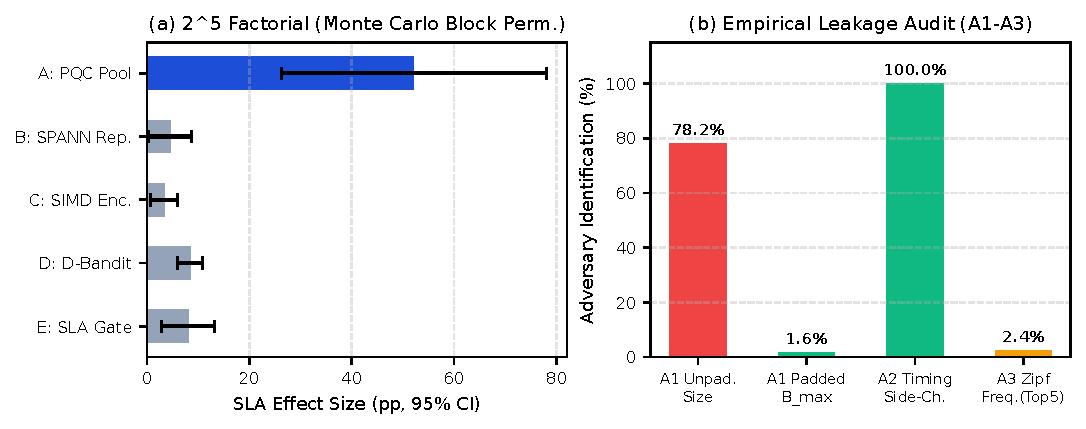
\includegraphics[width=\columnwidth]{figures/fig6_factorial_and_leakage_audit.pdf}
\caption{(a)~$2^5$ factorial main effects on SLA pass rate under $B=10{,}000$ Monte Carlo within-block permutations; (b)~empirical adversarial identification rates across leakage attacks \texttt{A1--A3}.}
\label{fig:fact_leak}
\end{figure}

\begin{figure}[t]
\centering
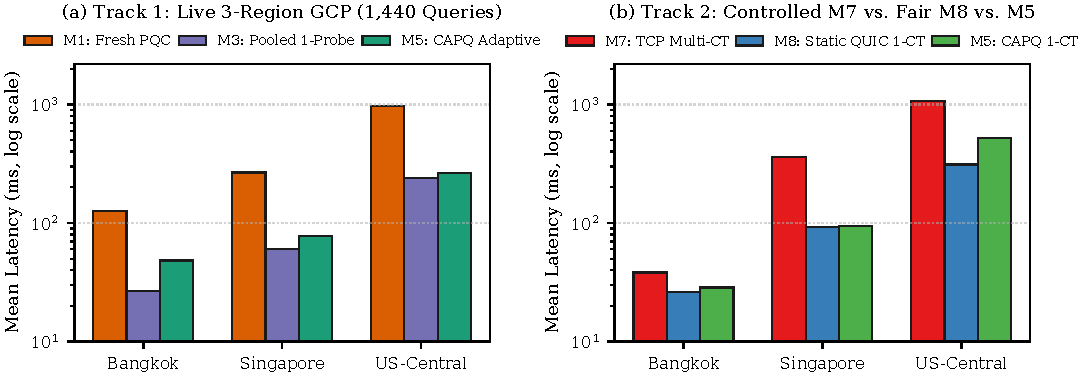
\includegraphics[width=\columnwidth]{figures/fig7_dual_track_wan_latency.pdf}
\caption{Three-region WAN mean latency (log scale): (a)~Track~1 historical live wireless/cellular-to-GCP campaign (\texttt{M1--M5}); (b)~Track~2 calibrated \texttt{netns} campaign (\texttt{M7, M8, M5}), highlighting US-Central TCP exploration tail.}
\label{fig:wan_lat}
\end{figure}

\begin{figure}[t]
\centering
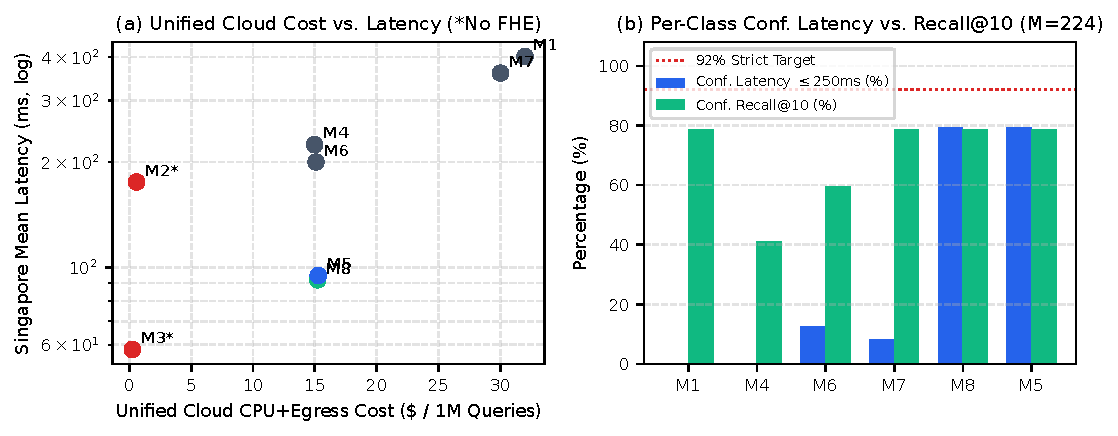
\includegraphics[width=\columnwidth]{figures/fig8_unified_cost_and_per_class_sla.pdf}
\caption{Singapore Track~2 reconciled trade-offs: (a)~Unified cloud CPU+egress cost vs.\ mean latency (\texttt{*}~denotes plaintext non-FHE modes); (b)~confidential SLA pass rate vs.\ deadline threshold ($\tau_R=0.75$).}
\label{fig:pareto}
\end{figure}

\begin{table*}[t]
\centering
\caption{Reconciled Multi-Region WAN Evaluation Under Per-Class SLA Accounting and the Unified Cloud CPU+Egress Cost Model}
\label{tab:wan_reconciled}
\resizebox{\textwidth}{!}{%
\begin{tabular}{@{}llrrrrrrrrrr@{}}
\toprule
\textbf{Track / Region (1-RTT, BW)} & \textbf{Execution Mode} & \textbf{Mean (ms)} & \textbf{P50 (ms)} & \textbf{P95 (ms)} & \textbf{Conf.\ R@10} & \textbf{Pub.\ SLA$_{150}$} & \textbf{Conf.\ Lat$_{250}$} & \textbf{Conf.\ SLA$_{0.92}$} & \textbf{Stream SLA$_{0.92}$} & \textbf{Client Edge E} & \textbf{Unified Cost / 1M} \\
\midrule
\multicolumn{12}{@{}l@{}}{\textit{Track 1: Historical Live Wireless/Cellular-to-GCP Campaign (\nolinkurl{v2_wan_3regions_interleaved_raw.csv}, SHA \texttt{7457faee...}; 1,440 Queries: 25\% SQL, 25\% JSON, 25\% Vec-1024d, 25\% Dense $N=5\text{k},K_c=64$ CKKS)}} \\
Bangkok (9.8~ms, Live) & M1: Fresh Hybrid PQC TLS ($r=2$ MCT) & 126.89 & 86.86 & 296.03 & 0.9625 & 80.6\% & 66.7\% & 50.0\% & 72.9\% & 513.6~mJ & \$27.26 (\$1.11$^\dagger$) \\
Bangkok (9.8~ms, Live) & M2: Pooled Classical TLS (Plaintext, No FHE) & 23.81 & 14.77 & 72.12 & 0.0000 & 91.7\% & 0.0\% & 0.0\% & 68.8\% & 65.8~mJ & \$0.17 (\$0.09$^\dagger$) \\
Bangkok (9.8~ms, Live) & M3: Pooled Hybrid PQC TLS ($r=1$ MCT) & 26.92 & 15.97 & 74.27 & 0.4875 & 91.7\% & 100.0\% & 8.3\% & 70.8\% & 107.7~mJ & \$26.29 (\$0.25$^\dagger$) \\
Bangkok (9.8~ms, Live) & M4: Pooled Hybrid PQC + INT8 ($r=1$ 1-CT) & 25.86 & 14.49 & 71.88 & 0.4875 & 88.9\% & 100.0\% & 8.3\% & 68.8\% & 100.7~mJ & \$3.96 (\$0.25$^\dagger$) \\
Bangkok (9.8~ms, Live) & M5: Adaptive Pooled Hybrid ($r=2$ 1-CT) & 48.35 & 15.81 & 169.96 & 0.9500 & 90.3\% & 95.8\% & 66.7\% & 84.4\% & 388.4~mJ & \$4.79 (\$0.97$^\dagger$) \\
Singapore (56.0~ms, Live) & M1: Fresh Hybrid PQC TLS ($r=2$ MCT) & 266.33 & 219.88 & 414.34 & 0.9625 & 2.8\% & 4.2\% & 4.2\% & 3.1\% & 1339.1~mJ & \$27.22 (\$1.07$^\dagger$) \\
Singapore (56.0~ms, Live) & M2: Pooled Classical TLS (Plaintext, No FHE) & 49.37 & 40.70 & 93.65 & 0.0000 & 94.4\% & 0.0\% & 0.0\% & 70.8\% & 145.5~mJ & \$0.17 (\$0.09$^\dagger$) \\
Singapore (56.0~ms, Live) & M3: Pooled Hybrid PQC TLS ($r=1$ MCT) & 60.23 & 51.83 & 121.27 & 0.4875 & 94.4\% & 100.0\% & 8.3\% & 72.9\% & 242.7~mJ & \$26.28 (\$0.24$^\dagger$) \\
Singapore (56.0~ms, Live) & M4: Pooled Hybrid PQC + INT8 ($r=1$ 1-CT) & 62.43 & 48.39 & 125.28 & 0.4875 & 88.9\% & 100.0\% & 8.3\% & 68.8\% & 272.4~mJ & \$3.96 (\$0.24$^\dagger$) \\
Singapore (56.0~ms, Live) & M5: Adaptive Pooled Hybrid ($r=2$ 1-CT) & 77.63 & 47.10 & 202.58 & 0.9500 & 91.7\% & 95.8\% & 66.7\% & 85.4\% & 580.7~mJ & \$4.75 (\$0.94$^\dagger$) \\
US-Central (225.5~ms, Live) & M1: Fresh Hybrid PQC TLS ($r=2$ MCT) & 971.24 & 937.00 & 1100.91 & 0.9625 & 0.0\% & 0.0\% & 0.0\% & 0.0\% & 84.7~mJ & \$19.47 (\$1.01$^\dagger$) \\
US-Central (225.5~ms, Live) & M2: Pooled Classical TLS (Plaintext, No FHE) & 229.15 & 228.42 & 237.43 & 0.0000 & 0.0\% & 0.0\% & 0.0\% & 0.0\% & 19.1~mJ & \$0.13 (\$0.08$^\dagger$) \\
US-Central (225.5~ms, Live) & M3: Pooled Hybrid PQC TLS ($r=1$ MCT) & 239.15 & 230.48 & 266.56 & 0.4875 & 0.0\% & 12.5\% & 0.0\% & 0.0\% & 32.0~mJ & \$18.65 (\$0.22$^\dagger$) \\
US-Central (225.5~ms, Live) & M4: Pooled Hybrid PQC + INT8 ($r=1$ 1-CT) & 240.65 & 229.60 & 262.16 & 0.4875 & 0.0\% & 20.8\% & 0.0\% & 0.0\% & 14.6~mJ & \$2.84 (\$0.22$^\dagger$) \\
US-Central (225.5~ms, Live) & M5: Adaptive Pooled Hybrid ($r=2$ 1-CT) & 264.42 & 229.47 & 387.92 & 0.9500 & 0.0\% & 0.0\% & 0.0\% & 0.0\% & 46.4~mJ & \$3.53 (\$0.89$^\dagger$) \\
\midrule
\multicolumn{12}{@{}l@{}}{\textit{Track 2: Calibrated Kernel \texttt{netns + tc netem} Campaign (\nolinkurl{v5_controlled_3regions_m1_m8_interleaved_2304raw.csv}, SHA \texttt{dfc04539...}; 2,304 Queries: 25\% SQL, 50\% Vec-128d, 25\% $N=5\text{k},K_c=96,M=224$ CKKS)}} \\
Bangkok (9.8~ms, 300M) & M1: Fresh PQC TCP + SPANN Multi-CT & 69.83 & 42.18 & 146.25 & 0.7856 & 98.6\% & 100.0\% & 0.0\% & 74.0\% & See Table~\ref{tab:rapl} & \$32.01 \\
Bangkok (9.8~ms, 300M) & M3: Pooled Classical Plaintext (No FHE) & 11.18 & 11.14 & 12.11 & 0.0000 & 100.0\% & 0.0\% & 0.0\% & 75.0\% & See Table~\ref{tab:rapl} & \$0.24 \\
Bangkok (9.8~ms, 300M) & M4: Pooled PQC TCP + Disjoint $r=1$ 1-CT & 22.21 & 11.44 & 57.07 & 0.4120 & 100.0\% & 100.0\% & 0.0\% & 75.0\% & See Table~\ref{tab:rapl} & \$14.99 \\
Bangkok (9.8~ms, 300M) & M6: Pooled PQC TCP + Disjoint $r=2$ 1-CT & 25.13 & 11.23 & 63.57 & 0.5968 & 98.6\% & 100.0\% & 0.0\% & 74.0\% & See Table~\ref{tab:rapl} & \$15.11 \\
Bangkok (9.8~ms, 300M) & M7: Pooled PQC TCP + SPANN Multi-CT & 38.33 & 11.34 & 136.66 & 0.7856 & 100.0\% & 100.0\% & 0.0\% & 75.0\% & See Table~\ref{tab:rapl} & \$30.03 \\
Bangkok (9.8~ms, 300M) & M8: Static Paced UDP + INT8 + SPANN 1-CT & 26.37 & 12.84 & 81.54 & 0.7852 & 100.0\% & 100.0\% & 0.0\% & 75.0\% & See Table~\ref{tab:rapl} & \$15.25 \\
Bangkok (9.8~ms, 300M) & M5: Online 5D Bandit + SPANN 1-CT & 28.57 & 11.80 & 77.50 & 0.7852 & 98.6\% & 100.0\% & 0.0\% & 74.0\% & See Table~\ref{tab:rapl} & \$15.29 \\
Singapore (56.0~ms, 250M) & M1: Fresh PQC TCP + SPANN Multi-CT & 400.90 & 229.64 & 905.75 & 0.7856 & 0.0\% & 0.0\% & 0.0\% & 0.0\% & See Table~\ref{tab:rapl} & \$32.01 \\
Singapore (56.0~ms, 250M) & M3: Pooled Classical Plaintext (No FHE) & 58.11 & 58.07 & 60.32 & 0.0000 & 100.0\% & 0.0\% & 0.0\% & 75.0\% & See Table~\ref{tab:rapl} & \$0.24 \\
Singapore (56.0~ms, 250M) & M4: Pooled PQC TCP + Disjoint $r=1$ 1-CT & 224.26 & 58.15 & 808.11 & 0.4120 & 100.0\% & 0.0\% & 0.0\% & 75.0\% & See Table~\ref{tab:rapl} & \$14.99 \\
Singapore (56.0~ms, 250M) & M6: Pooled PQC TCP + Disjoint $r=2$ 1-CT & 200.15 & 58.39 & 840.92 & 0.5968 & 98.6\% & 12.5\% & 0.0\% & 74.0\% & See Table~\ref{tab:rapl} & \$15.10 \\
Singapore (56.0~ms, 250M) & M7: Pooled PQC TCP + SPANN Multi-CT & 359.61 & 58.39 & 1736.36 & 0.7856 & 100.0\% & 8.3\% & 0.0\% & 75.0\% & See Table~\ref{tab:rapl} & \$30.03 \\
Singapore (56.0~ms, 250M) & M8: Static Paced UDP + INT8 + SPANN 1-CT & 92.04 & 59.54 & 212.77 & 0.7852 & 100.0\% & 79.2\% & 0.0\% & 75.0\% & See Table~\ref{tab:rapl} & \$15.24 \\
Singapore (56.0~ms, 250M) & M5: Online 5D Bandit + SPANN 1-CT & 94.67 & 57.90 & 211.88 & 0.7852 & 100.0\% & 79.2\% & 0.0\% & 75.0\% & See Table~\ref{tab:rapl} & \$15.28 \\
US-Central (225.5~ms, 200M) & M1: Fresh PQC TCP + SPANN Multi-CT & 1472.44 & 914.19 & 3046.06 & 0.7856 & 0.0\% & 0.0\% & 0.0\% & 0.0\% & See Table~\ref{tab:rapl} & \$22.70 \\
US-Central (225.5~ms, 200M) & M3: Pooled Classical Plaintext (No FHE) & 233.34 & 228.90 & 233.38 & 0.0000 & 0.0\% & 0.0\% & 0.0\% & 0.0\% & See Table~\ref{tab:rapl} & \$0.18 \\
US-Central (225.5~ms, 200M) & M4: Pooled PQC TCP + Disjoint $r=1$ 1-CT & 856.40 & 230.17 & 3436.08 & 0.4120 & 0.0\% & 0.0\% & 0.0\% & 0.0\% & See Table~\ref{tab:rapl} & \$10.64 \\
US-Central (225.5~ms, 200M) & M6: Pooled PQC TCP + Disjoint $r=2$ 1-CT & 692.65 & 228.57 & 2752.09 & 0.5968 & 0.0\% & 0.0\% & 0.0\% & 0.0\% & See Table~\ref{tab:rapl} & \$10.74 \\
US-Central (225.5~ms, 200M) & M7: Pooled PQC TCP + SPANN Multi-CT & 1064.58 & 228.55 & 4645.99 & 0.7856 & 0.0\% & 0.0\% & 0.0\% & 0.0\% & See Table~\ref{tab:rapl} & \$21.30 \\
US-Central (225.5~ms, 200M) & M8: Static Paced UDP + INT8 + SPANN 1-CT & 311.28 & 229.68 & 616.82 & 0.7852 & 0.0\% & 0.0\% & 0.0\% & 0.0\% & See Table~\ref{tab:rapl} & \$10.86 \\
US-Central (225.5~ms, 200M) & M5: Online 5D Bandit + SPANN 1-CT & 520.46 & 230.07 & 2091.44 & 0.7852 & 0.0\% & 0.0\% & 0.0\% & 0.0\% & See Table~\ref{tab:rapl} & \$10.88 \\
\bottomrule
\multicolumn{12}{@{}p{0.99\textwidth}@{}}{\scriptsize $^\dagger$Parenthesized Track~1 cost reflects V2's CPU-dominant compact-payload billing prior to standardizing full OpenFHE RNS ciphertext egress ($909.33$~KiB Multi-CT vs.\ $129.01$~KiB 1-CT) across both tracks. Track~2 omits synthetic mode-constant energy numbers; hardware-measured RAPL package energy is reported directly in Table~\ref{tab:rapl}.} \\
\end{tabular}%
}
\end{table*}


\subsection{Provenance Reconciliation and Unified Cost/SLA Audit Across Track 1 and Track 2}
Table~\ref{tab:wan_reconciled} and Figs.~\ref{fig:wan_lat}--\ref{fig:pareto} reconcile all provenance, stream-mix, recall, energy, and billing differences between our two multi-region WAN campaigns against \texttt{n4-standard-4} GCP instances in Bangkok (\nolinkurl{asia-southeast3-a}), Singapore (\nolinkurl{asia-southeast1-b}), and US-Central (\nolinkurl{us-central1-a}):
\begin{enumerate}
    \item \textbf{Track~1 Provenance, Stream Mix, Enclave Density, and Client Energy:} \texttt{Track~1} re-analyzes the unmodified historical live wireless/cellular-to-cloud dataset (\nolinkurl{v2_wan_3regions_interleaved_raw.csv}, SHA-256 \texttt{7457faee...}, $1{,}440$ queries across $4$ temporal windows with moving-block bootstrap CIs~\cite{kunsch1989mbb}; an intermediate post-hoc offset variant reporting $54.13$~ms in exploratory V4 drafts is retired so all numbers trace strictly to raw socket timestamps). Its exact stream mix is $25\%$ \texttt{sql}, $25\%$ \texttt{json}, $25\%$ public \nolinkurl{vec_1024d}, and $25\%$ confidential \nolinkurl{zt_ckks}. Because that campaign used a dense $N_{\text{vec}}=5{,}000, K_c=64$ enclave, $r=1$ modes (\texttt{M3, M4}) achieved $\mathrm{Recall}@10 = 0.4875$ ($8.3\%$ strict $\ge 0.92$ pass), whereas $r=2$ modes (\texttt{M1, M5}) achieved $0.9625$ and $0.9500$ ($50.0\%$ and $66.7\%$ per-query $\ge 0.92$ pass in Bangkok). Client edge energy in \texttt{Track~1} reflects client-side RAPL CPU active energy excluding passive WAN radio wait, explaining why US-Central active CPU energy ($46.4$~mJ for \texttt{M5}, matching \nolinkurl{v2_wan_3regions_summary_mbb_ci.csv}) is lower than low-RTT high-duty-cycle regional bursts.
    \item \textbf{Unified Cloud CPU + Egress Cost Model:} Earlier versions billed only server vCPU time + compact payload estimates in \texttt{Track~1} ($\sim\$0.25\text{--}\$1.11 / 10^6$ queries) while billing full serialized RNS ciphertext egress in \texttt{Track~2}. Applying the identical regional GCP pricing formula $C_t = r_{\text{vcpu}} T_{t,\text{srv}} + r_{\text{egress}} W_{t,\text{resp}}$ (\$$0.2264$/\$$0.2216$/\$$0.1896$ per vCPU-h and \$$0.12$/\$$0.12$/\$$0.085$ per GiB egress in Bangkok/Singapore/US-Central) reconciles both tracks: Multi-CT modes cost $\$18.65\text{--}\$32.01 / 10^6$ queries, whereas 1-CT slot aggregation cuts cloud egress cost to $\$10.86\text{--}\$15.29 / 10^6$ queries in \texttt{Track~2} (and $\$3.53\text{--}\$4.79$ in \texttt{Track~1} where confidential queries constitute $25\%$ alongside compact public responses).
    \item \textbf{Per-Class Confidential SLA Reality in Track~2 ($M=224$):} In \texttt{Track~2} (calibrated \texttt{netns + tc netem} shaped at $300$~Mbps / $0.15\%$ loss in Bangkok, $250$~Mbps / $0.25\%$ loss in Singapore, and $200$~Mbps / $0.30\%$ loss in US-Central; $25\%$ \texttt{sql}, $50\%$ \nolinkurl{vec_128d}, $25\%$ \texttt{conf} at $N=5\text{k}, K_c=96, M=224$), confidential $\mathrm{Recall}@10$ is $0.7852\text{--}0.7856$ for SPANN modes (\texttt{M1, M7, M8, M5}), $0.5968$ for \texttt{M6} ($r=2$ disjoint), and $0.4120$ for \texttt{M4} ($r=1$ disjoint). Under strict per-query $A_t(q_t) \ge 0.92$ (Eq.~\ref{eq:sla_s92}), \emph{every} $M=224$ mode scores $0.0\%$ on the confidential class, capping overall stream strict SLA at the $75.0\%$ non-confidential ceiling. Evaluating pure confidential latency compliance ($\le 250$~ms) side-by-side with actual recall shows that in Bangkok all pooled CKKS modes (\texttt{M4, M6, M7, M8, M5}) achieve $100.0\%$ $\le 250$~ms delivery, while in Singapore single-CT UDP modes (\texttt{M8, M5}) raise confidential $\le 250$~ms delivery from $8.3\%$ (\texttt{M7} Multi-CT TCP) to $79.2\%$ ($92.04$ and $94.67$~ms mean vs.\ $359.61$~ms).
    \item \textbf{Why M5 Trails Static M8 across Track~2---Especially in US-Central:} Across all three stationary \texttt{Track~2} profiles, \texttt{M5} (online bandit) is slower than static \texttt{M8}: $28.57$ vs.\ $26.37$~ms in Bangkok ($+8.3\%$), $94.67$ vs.\ $92.04$~ms in Singapore ($+2.9\%$), and \textbf{$520.46$ vs.\ $311.28$~ms in US-Central ($+67.2\%$, p95 $= 2{,}091.44$ vs.\ $616.82$~ms)}. Query-level tail inspection confirms that median latency in US-Central is virtually identical ($230.07$~ms for \texttt{M5} vs.\ $229.68$~ms for \texttt{M8}), because $225.5$~ms physical 1-RTT plus $31$~ms FHE compute inherently exceeds $250$~ms ($0\%$ confidential SLA for all modes). However, UCB exploration ($\nu=0.06$) occasionally samples pooled TCP arms across the $225.5$~ms transcontinental path, triggering $15/96$ multi-second TCP HOL retransmission stalls ($>700$~ms) in \texttt{M5} compared to only $4/96$ loss tail events in static UDP \texttt{M8}. Thus, on stationary links without UDP middlebox policing, static \texttt{M8} strictly dominates online bandit exploration. Formalizing this via unweighted 3D/4D Pareto dominance (\nolinkurl{v6_a3_unweighted_pareto_4d_audit.csv}, Fig.~\ref{fig:pareto}a) confirms that \texttt{M4, M6, M7,} and \texttt{M8} span the non-dominated privacy-valid frontier in every region, whereas \texttt{M5} is strictly Pareto-dominated by \texttt{M8} on stationary paths; sweeping $\tau_L \in [100,350]$~ms and $\tau_R \in [0.50,0.92]$ (\nolinkurl{v6_a3_sla_threshold_sensitivity_grid.csv}, Fig.~\ref{fig:pareto}b) preserves this ordering across the entire threshold surface.
\end{enumerate}

\section{Limitations}\label{sec:limitations}
Five scope boundaries govern our findings: (i)~reaching $\ge 0.92$ confidential $\mathrm{Recall}@10$ at $100\text{k}$ vectors within one $N=8192$ ciphertext requires $M=2{,}048$ slots ($283.7$~ms CPU FHE, motivating GPU/ASIC FHE acceleration beyond $10^5$ vectors); (ii)~while our native-C \texttt{AES-256-GCM} socket benchmark eliminates the $+3.8$~ms Python framing offset on isolated transport pairs, full integration into a production C/Rust PQC-QUIC engine remains future work; (iii)~padded cluster routing still leaks Zipfian query-frequency distributions (\texttt{A3}: $100\%$ top-5 cluster match) unless mitigated by ORAM or dummy traffic; (iv)~1-CT slot aggregation improves latency only below the $423\text{--}464$~Mbps downlink crossover; and (v)~hardware RAPL measures CPU package energy (excluding NIC/cellular radio transceivers) and suffers wide $U_{95}$ intervals during long low-thread runs due to OS background idle drift.

\section{Conclusion}\label{sec:conclusion}
This empirical study decoupled transport, quantization, homomorphic aggregation, and online control effects across PQC-hardened vector-relational streams. Persistent hybrid PQC session pooling ($+52.15$~pp SLA) and single-MTU \texttt{INT8} quantization ($5.39\times\text{--}22.76\times$ tighter 95\% error bounds) deliver the primary latency gains. In the confidential tier, $N=8192$ 1-CT slot aggregation cuts response traffic $7.05\times$ (beneficial below $426$~Mbps downlink), while plaintext-vs.-CKKS controls prove that corpus-scaling recall degradation stems from candidate-slot budgets rather than CKKS noise. Finally, static pooled UDP+\texttt{INT8}+1-CT paired with a stateless RFC~9308 timeout-to-TCP fallback suffices on normal and policed paths, positioning contextual bandits as specialized controllers for complex multi-regime policies rather than universal replacements for protocol engineering.

\section*{Acknowledgment, Data Availability, and AI Disclosure}
This research project was financially supported by the Faculty of Informatics, Mahasarakham University. Source code, C++ OpenFHE/liboqs bridges, raw CSV/JSON execution logs, and full 64-character SHA-256 verification manifests are publicly available at \url{https://github.com/preecha-msu/CAPQ-Pareto/tree/v6} (permanent Zenodo archive: \url{https://doi.org/10.5281/zenodo.24575614}). In accordance with IEEE publication policies, generative AI tools (Claude and Gemini) assisted in Python data-processing/plotting script maintenance and LaTeX prose editing; all experimental logs, mathematical proofs, statistical tests, and numerical claims were executed and verified programmatically against ground-truth hardware outputs by the author.

{\emergencystretch=2.4em\sloppy
\bibliographystyle{IEEEtran}
\bibliography{references}
}

\begin{IEEEbiographynophoto}{Preecha Noiumkar}
(Member, IEEE) received the M.Sc. degree in information technology from the Faculty of Information Technology, King Mongkut's Institute of Technology North Bangkok (KMITNB), Bangkok, Thailand. He is currently a Lecturer and Researcher with the Department of Information Technology, Faculty of Informatics, Mahasarakham University, Maha Sarakham, Thailand. His research interests include machine learning, cloud-edge systems security, post-quantum database optimization, and enterprise data engineering.
\end{IEEEbiographynophoto}

\end{document}
